\documentclass{article}
\usepackage{xeCJK}
\usepackage{amsmath}
\usepackage{amssymb}
\usepackage{mathrsfs}
\usepackage{bm}
\usepackage{hyperref}
\usepackage{graphicx}
\usepackage{subcaption}
\usepackage{float}
\usepackage[ruled,linesnumbered]{algorithm2e}

\setlength{\parindent}{2em}
\usepackage{geometry}
\geometry{a4paper, left=2.54cm, right=2.54cm, top=3.18cm, bottom=3.18cm}

% 设置文章行距
\renewcommand{\baselinestretch}{1.5}

% 定义引用格式
% \newcommand{\myeqref}[1]{\eqref{#1}式}
% \newcommand{\figref}[1]{图\ref{#1}}
% \newcommand{\tabref}[1]{表\ref{#1}}

\begin{document}


\section{局部耦合中跨边界坐标的调整}\label{positionAdj}

\begin{figure}[htbp]
    \centering
    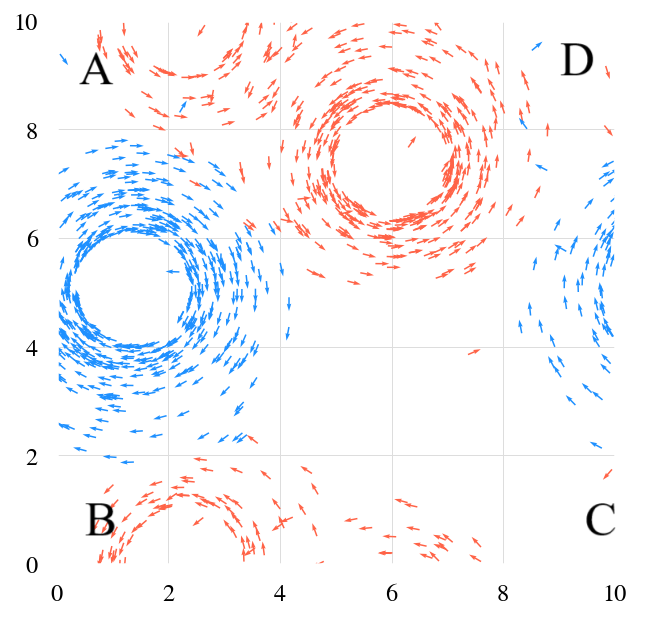
\includegraphics[width=0.4\textwidth]{./figs/fig1.jpg}
    \caption{跨边界坐标的调整}
    \label{fig:fig22}
\end{figure}

给定$(x_i, y_i)$, 对于任意的$(x_j, y_j)$, 做如下变换

\begin{equation}\label{eq:eq1}
	\bar{x}_j=\begin{cases}
		x_j,&		|x_i-x_j|\le L/2\\
		x_j+L,&		x_i-x_j>L/2\\
		x_j-L,&		x_j-x_i>L/2\\
	\end{cases} ,\quad
	\bar{y}_j=\begin{cases}
		y_j,&		|y_i-y_j|\le L/2\\
		y_j+L,&		y_i-y_j>L/2\\
		y_j-L,&		y_j-y_i>L/2\\
	\end{cases}
\end{equation}

其中,$L$为边界长度. 例如,对于\ref{fig:fig22}中的情况,以A为$(x_i, y_i)$时,B需调整纵坐标,D需调整横坐标,C需同时调整横纵坐标.

$\ $

原始距离为

$$
d_{ij}=\sqrt{(x_i-x_j)^2+(y_i-y_j)^2}
$$

变换后的距离为

$$
\bar{d}_{ij}=\sqrt{(x_i-\bar{x}_j)^2+(y_i-\bar{y}_j)^2}
$$

下证$\bar{d}_{ij} \le d_{ij}$, 即调整后的距离不会大于原始距离.

$ $

对于$(x_i-x_j)^2, (x_i-\bar{x}_j)^2$, 若$x_i\ne \bar{x}_j$,有

$$
\begin{array}{l}
	(x_i-\bar{x}_j)^2-(x_i-x_j)^2\\
	=\left( x_j\pm L-x_i \right) ^2-(x_i-x_j)^2\\
	=L^2\pm 2L\left( x_j-x_i \right)\\
	=\left\{ \begin{matrix}
	L^2+2L\left( x_j-x_i \right) ,&		x_i-x_j>5\\
	L^2-2L\left( x_j-x_i \right) ,&		x_j-x_i>5\\
\end{matrix} \right.\\
	<L^2-10L\\
	=0, \left( L=10 \right)\\
\end{array}
$$

即

$$
(x_i-\bar{x}_j)^2<(x_i-x_j)^2, \left( L=10, x_i\ne \bar{x}_j \right)
$$

同理可证

$$
(y_i-\bar{y}_j)^2<(y_i-y_j)^2, \left( L=10, x_i\ne \bar{x}_j \right)
$$

综上有

$$
\bar{d}_{ij}=\sqrt{(x_i-\bar{x}_j)^2+(y_i-\bar{y}_j)^2}\le \sqrt{(x_i-x_j)^2+(y_i-y_j)^2}=d_{ij}
$$

当且仅当$x_i=\bar{x}_j$且$y_i=\bar{y}_j$时,取等号.

因此

$$
\begin{aligned}
	D_{ij}&=\min \left\{ \sqrt{(x_i-\bar{x}_j)^2+(y_i-\bar{y}_j)^2},\sqrt{(x_i-x_j)^2+(y_i-y_j)^2} \right\}\\
	&=\sqrt{(x_i-\bar{x}_j)^2+(y_i-\bar{y}_j)^2}\\
\end{aligned}
$$

\newpage

\section{相位-取向关联的集群振子系统的动力学研究}

\textbf{$\Delta$ 聚焦点}
\begin{enumerate}
    \item 环态及其相变
    \item 环态的解域与相位同步的关系
    \item 数值结果的细致讨论, 分类
    \item 必要的理论分析与估计
\end{enumerate}

\subsection{单个粒子的运动问题(无相互作用)}

$$
\begin{cases}
	\begin{array}{c}
	\Delta x\left( t \right) =v\cos \theta \Delta t\\
	\Delta y\left( t \right) =v\sin \theta \Delta t\\
\end{array}\rightarrow \begin{array}{c}
	\dot{x}=v\cos \theta\\
	\dot{y}=v\sin \theta\\
\end{array}\\
	\dot{\theta}_i=\omega _i\rightarrow \theta _i\left( t \right) =\omega _it\\
	v=\sqrt{\dot{x}_{i}^{2}+\dot{y}_{i}^{2}}=v\left( constant \right)\\
\end{cases}
$$

\textbf{运动半径的求解}

$$
\begin{cases}
	x_i\left( t \right) =x_i\left( 0 \right) -\frac{v}{\omega _i}\sin \omega _it\\
	y_i\left( t \right) =y_i\left( 0 \right) -\frac{v}{\omega _i}\cos \omega _it\\
\end{cases}
$$

$$
\Rightarrow \left( x_i-x_{i}^{0} \right) ^2+\left( y_i-y_{i}^{0} \right) ^2=\left( \frac{v}{\omega _i} \right) ^2
$$

每个粒子的运动轨迹是一个圆,圆心为 $\left( x_i^0,y_i^0 \right)$,半径为 $\frac{v}{\omega _i}$

\begin{figure}[H]
	\centering
	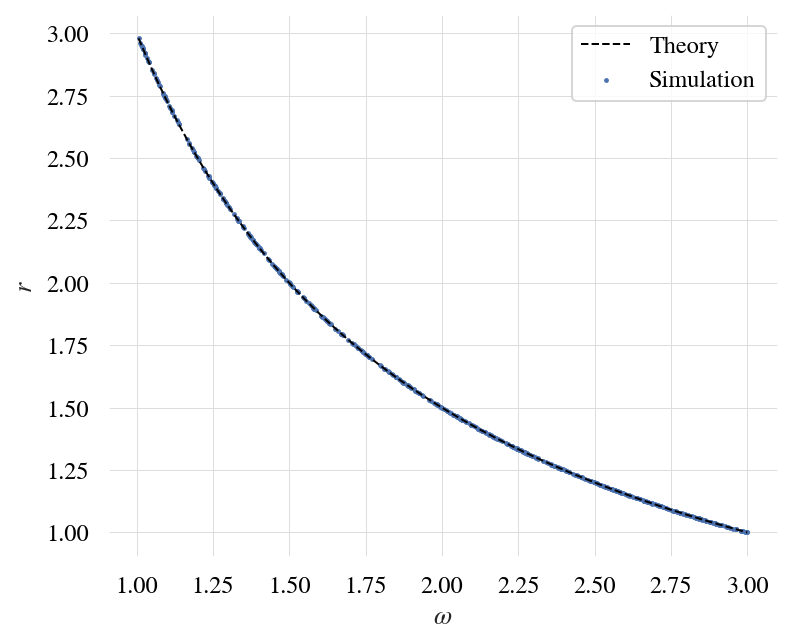
\includegraphics[width=0.5\textwidth]{./figs/noCouplingRadius.png}
	\caption{解析解与数值模拟结果 ($\lambda=0, d_0=0, random seed=10$, Single Chirality)}
	\label{fig:fig21.1}
\end{figure}

\begin{figure}[H]
	\centering
	\begin{subfigure}[b]{0.49\textwidth}
		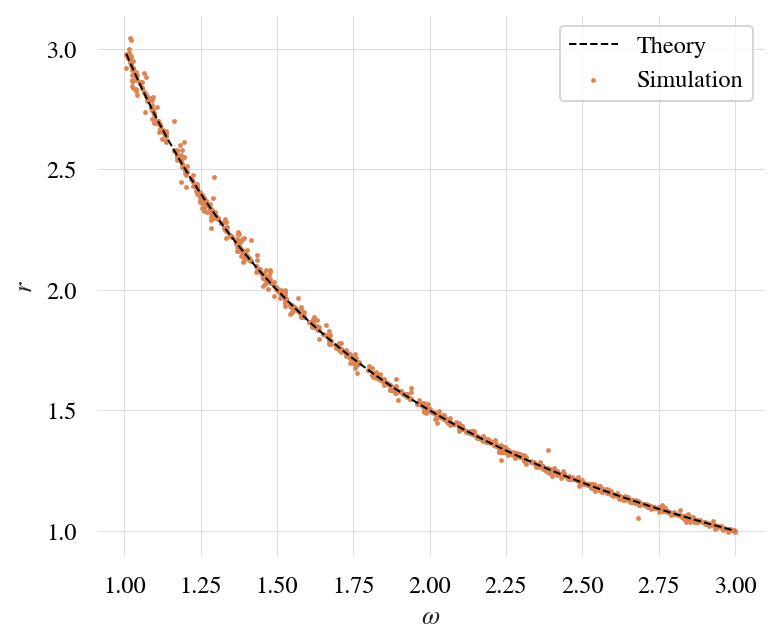
\includegraphics[width=\textwidth]{./figs/DisorderStateRadius.png}
		\vspace{-1cm}
		\caption{无序态 ($\lambda=0.01:0.03$)}
	\end{subfigure}
	% \hfill
	\begin{subfigure}[b]{0.49\textwidth}
		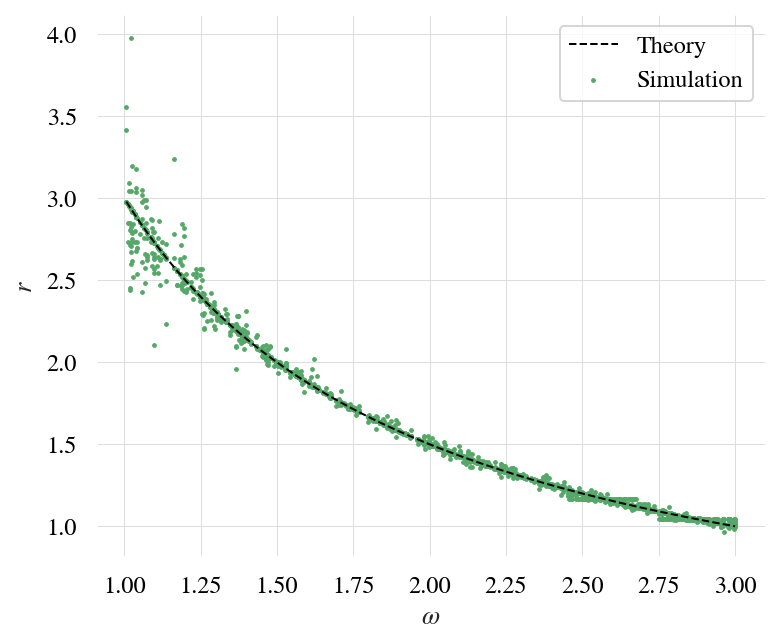
\includegraphics[width=\textwidth]{./figs/RingStateRadios.png}
		\vspace{-1cm}
		\caption{环态 ($\lambda=0.04:0.1$)}
	\end{subfigure}
	\vspace{-0.5cm}
	\caption{无序态、环态解析解与数值模拟结果 ($d_0=0.1, random seed=10$ Single Chirality)}
	\label{fig:fig21.2}
\end{figure}

% SwarmStateRadius.png
\begin{figure}[H]
	\centering
	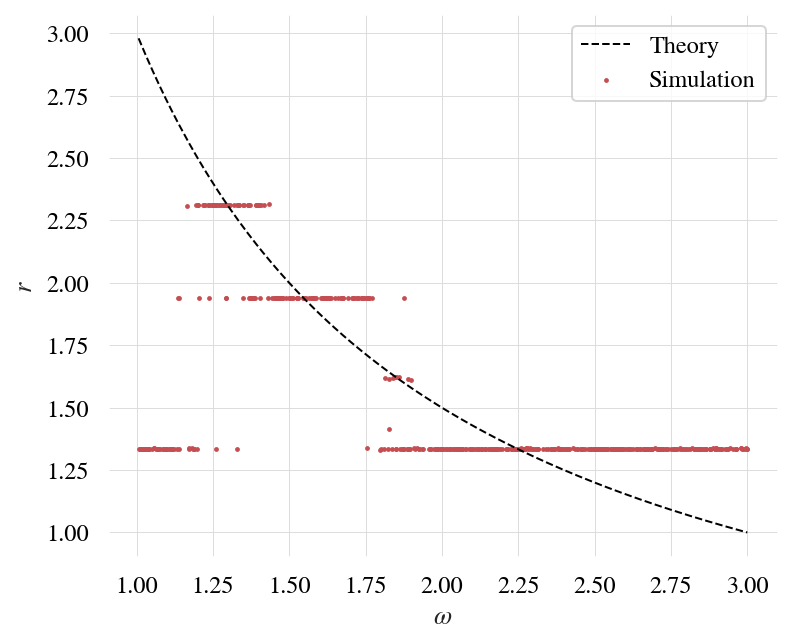
\includegraphics[width=0.5\textwidth]{./figs/SwarmStateRadius.png}
	\caption{集群态解析解与数值模拟结果 ($\lambda=0.1, d_0=0.3, random seed=10$, Single Chirality)}
	\label{fig:fig21.3}
\end{figure}


\subsection{考虑相互作用$\lambda$,耦合距离$d_0$ ($\{A_ij\}$,注意是时变的)}

\begin{itemize}
    \item 看空间聚集过程
    \item 空间尺度也考虑进去
\end{itemize}

粒子数$N$,$L\times L\sim \sqrt{\frac{L\times L}{N}}\sim \frac{L}{\sqrt{N}}$

\begin{enumerate}
    \item 每个单粒子的运动空间尺度, $\cfrac{v}{\omega_i}$
    \item 耦合距离 $d_0$
    \item 粒子平均间距 $\cfrac{L}{\sqrt{N}}$
\end{enumerate}

$$
d_0\sim \frac{L}{\sqrt{N}}\rightarrow d_0\ll \frac{L}{\sqrt{N}}, d_0\gg \frac{L}{\sqrt{N}}
$$

低频粒子:$d_0\ll \frac{v}{\omega _i}$
高频粒子:$d_0\gg \frac{v}{\omega _i}$

在计算空间pattern同时,还要跟踪每个粒子的相速度$\dot{\theta}_i(t)$

\subsection{序参量 Order Parameter}

\subsubsection{相位单位圆}

由于粒子数较多,为了更清晰地刻画粒子相位的同步情况,绘制三维空间中的单位圆. 将单位圆等分为$M$个区间,每个区间的大小为$\frac{2\pi}{M}$,$z$轴表示单位圆上相位处于该区间的粒子数,类似于分布.

\begin{figure}[H]
	\centering
	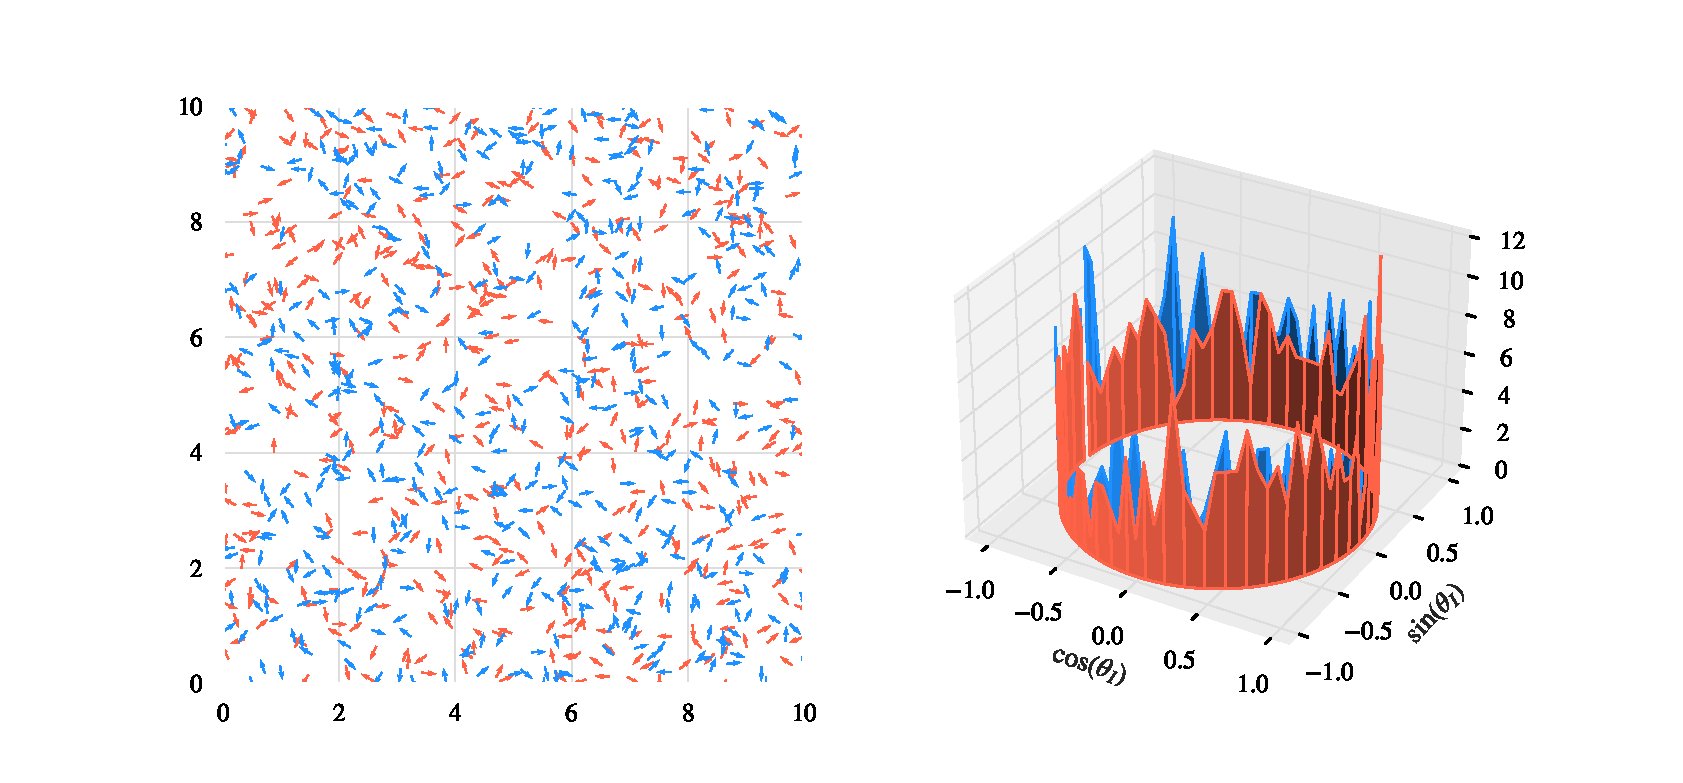
\includegraphics[width=\textwidth]{./figs/CorrectCoupling_uniform_0.010_0.10.eps}
	\vspace{-1cm}
	\caption{无序态 ($\lambda=0.01, d_0=0.1, random seed=10$)}
	\label{fig:fig231.1}
\end{figure}

\begin{figure}[H]
	\centering
	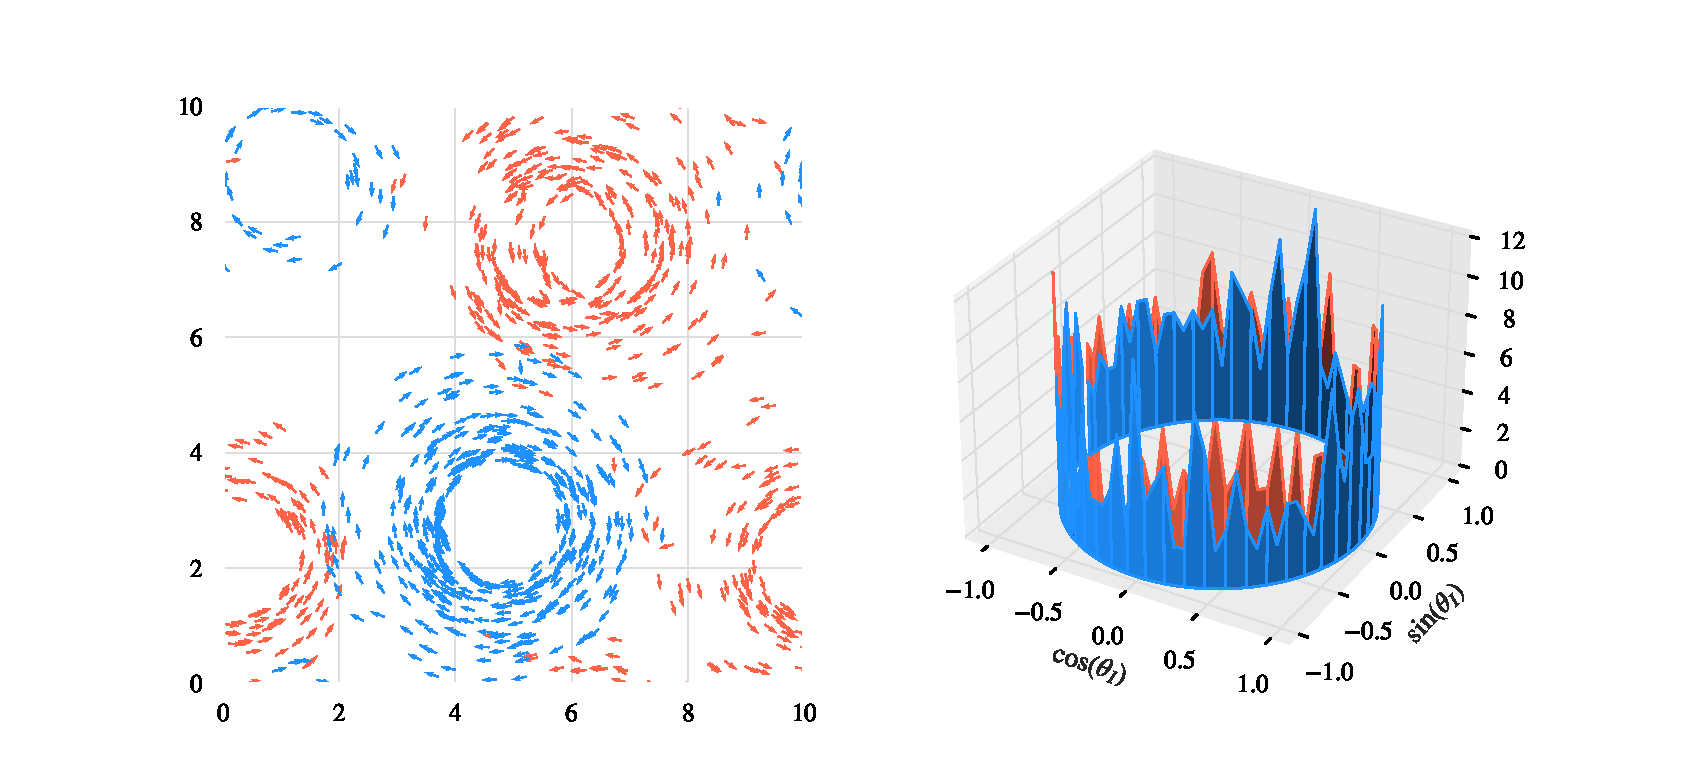
\includegraphics[width=\textwidth]{./figs/CorrectCoupling_uniform_0.020_0.30.eps}
	\vspace{-1cm}
	\caption{环态 ($\lambda=0.02, d_0=0.3, random seed=10$)}
	\label{fig:fig231.2}
\end{figure}

当粒子处于无序态或环态时,相位单位圆的分布如图\ref{fig:fig231.1}和图\ref{fig:fig231.2}所示. 此时,单位圆分布较为平滑,单位圆上的粒子数分布较为均匀, 相位同步的程度较低.

\begin{figure}[H]
	\centering
	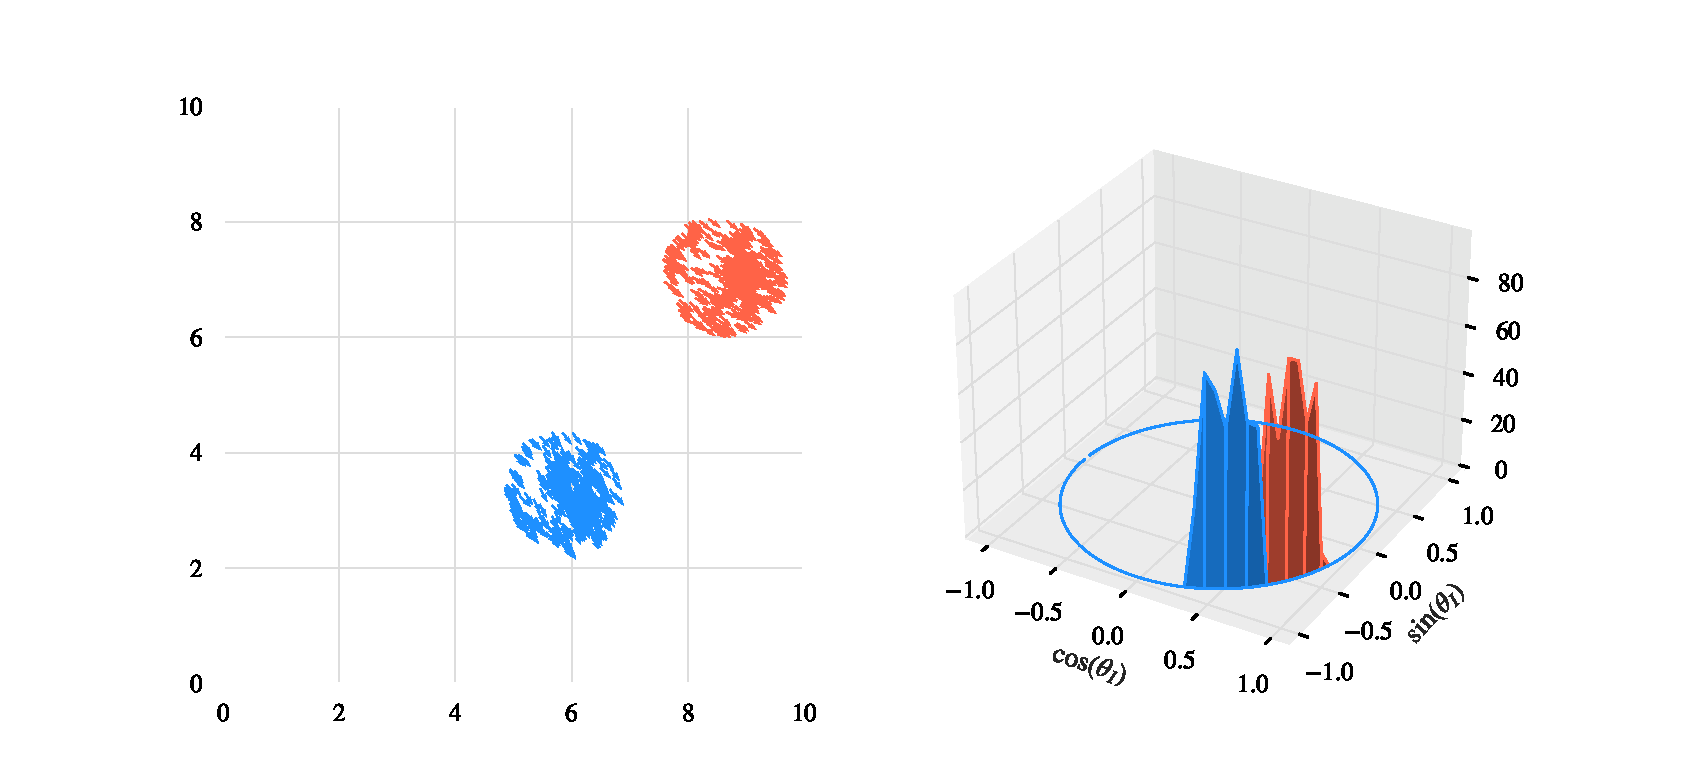
\includegraphics[width=\textwidth]{./figs/CorrectCoupling_uniform_0.010_2.00.eps}
	\vspace{-1cm}
	\caption{集群态 ($\lambda=0.01, d_0=2, random seed=10$)}
	\label{fig:fig231.3}
\end{figure}

\begin{figure}[H]
	\centering
	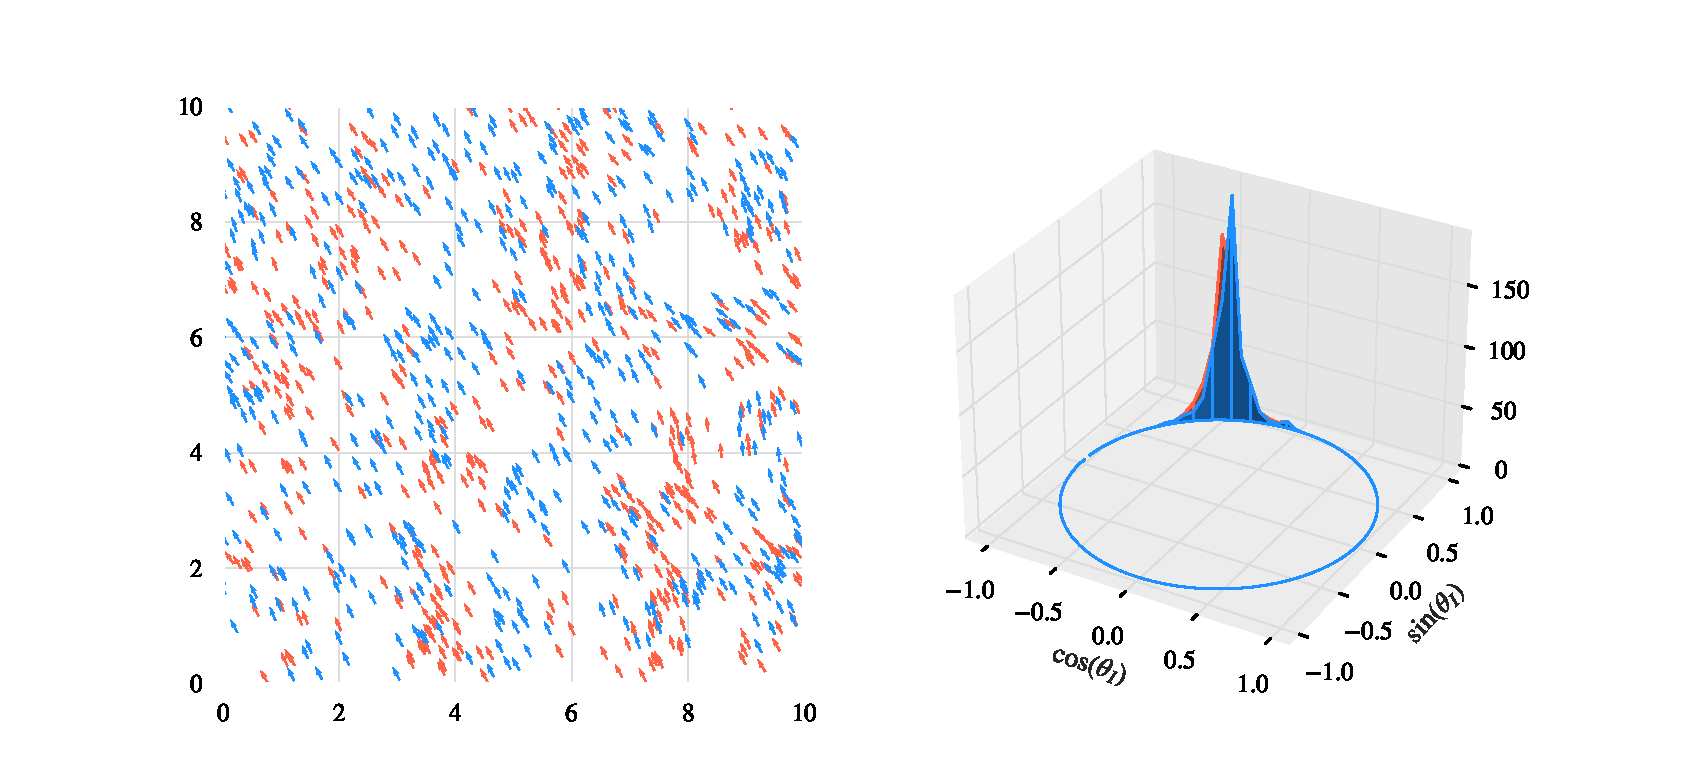
\includegraphics[width=\textwidth]{./figs/CorrectCoupling_uniform_0.600_3.00.eps}
	\vspace{-1cm}
	\caption{快速同步态 ($\lambda=0.6, d_0=3, random seed=10$)}
	\label{fig:fig231.4}
\end{figure}

当粒子处于集群态或快速同步态时,相位单位圆的分布如图\ref{fig:fig231.3}和图\ref{fig:fig231.4}所示. 这两种状态的相位同步的程度较高.

\subsubsection{粒子旋转中心的坐标}

\begin{figure}[H]
	\centering
	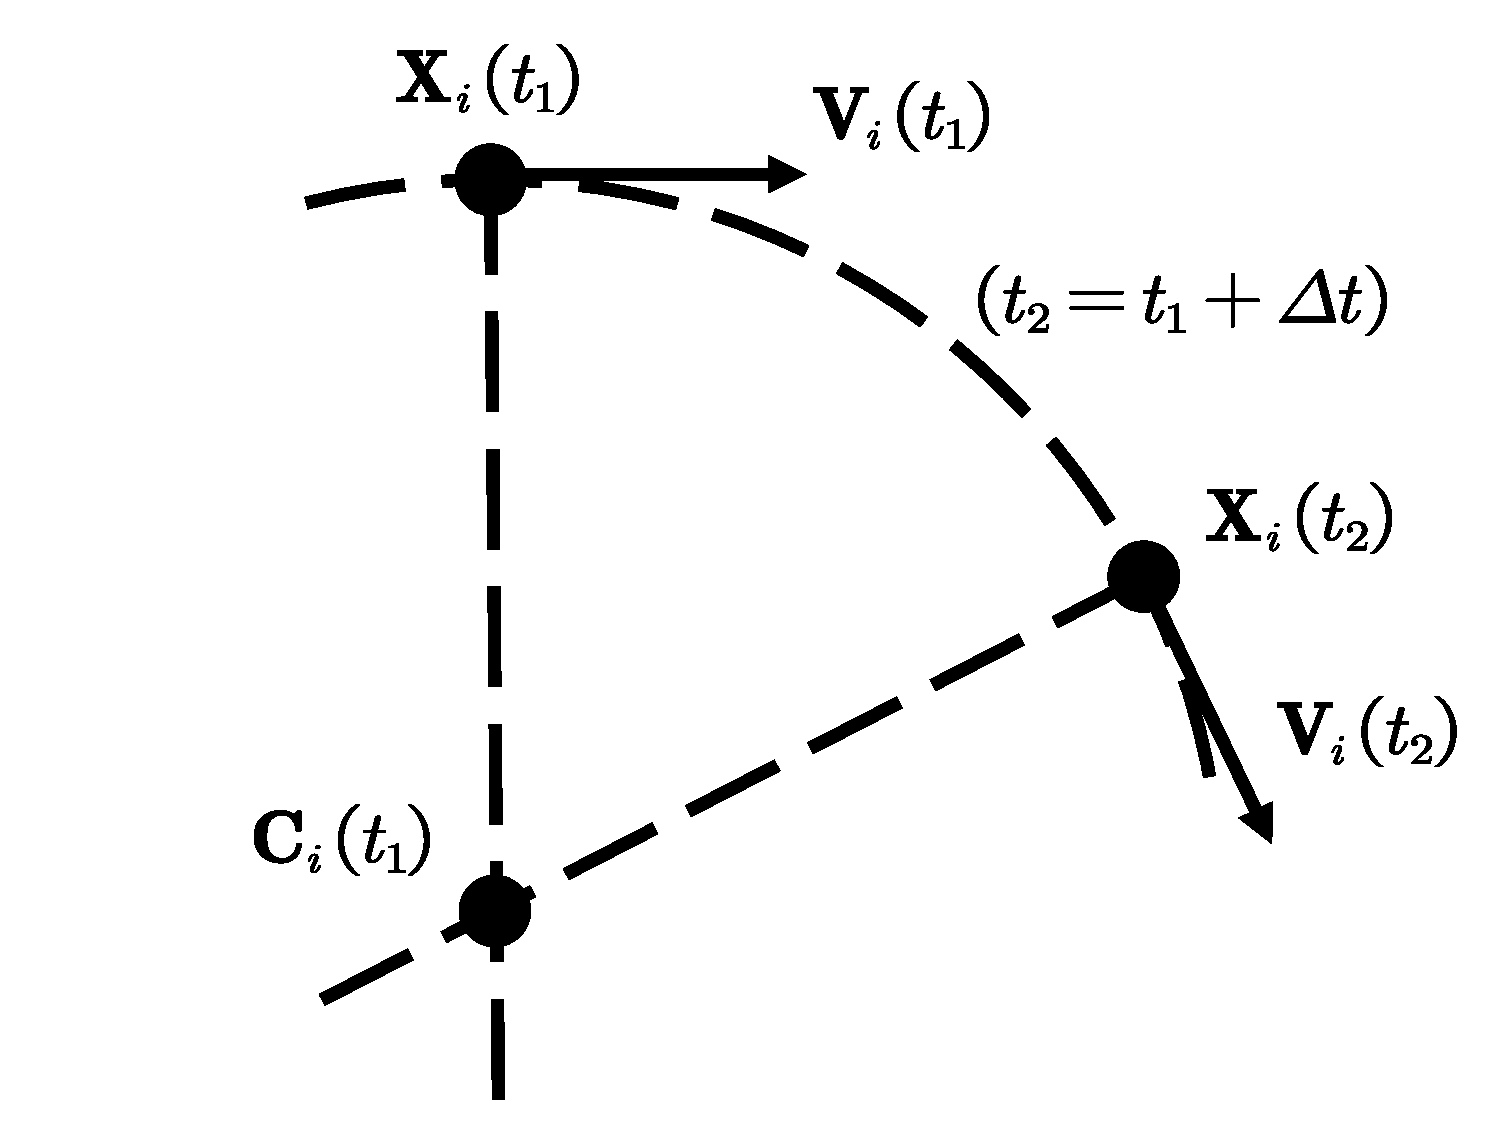
\includegraphics[width=0.3\textwidth]{./figs/CenterEps.pdf}
	\vspace{-0.2cm}
	\caption{旋转圆心示意图}
	\label{fig:fig232.1}
\end{figure}

如图 \ref{fig:fig232.1} 所示,对于任意粒子$i$, 其当前坐标为$\mathbf{X}_i\left( t_1 \right)$, 速度为$\mathbf{V}_i\left( t_1 \right)$, 下一时刻的坐标为$\mathbf{X}_i\left( t_2 \right)$, 速度为$\mathbf{V}_i\left( t_2 \right)$, 则其旋转中心坐标为两个时刻法向量所在直线的交点, 假设旋转中心坐标为$\mathbf{C}_i\left( t_1 \right)$, 则有

\vspace{-0.5cm}

$$
\begin{cases}
	\mathbf{C}_i\left( t_1 \right) \cdot \mathbf{V}_i\left( t_1 \right) =\mathbf{X}_i\left( t_1 \right) \cdot \mathbf{V}_i\left( t_1 \right) \\
	\mathbf{C}_i\left( t_1 \right) \cdot \mathbf{V}_i\left( t_2 \right) =\mathbf{X}_i\left( t_2 \right) \cdot \mathbf{V}_i\left( t_2 \right) \\
\end{cases}
$$

% 对于任意的粒子$i$,其当前坐标为$\left( x_i,y_i \right)$,相速度为$\dot{\theta}_i$,假设从当前时刻开始,其相速度不变,即$\dot{\theta}_i$为常数,记录该粒子在一个周期($2\pi$)内的运动轨迹,即$2\pi / \dot{\theta}_i$时间内,以当前坐标$\left( x_i,y_i \right)$为起点,以$\left\{ v\cos \theta _i,v\sin \theta _i \right\} $为速度,运动得到的轨迹,以轨迹上点坐标的算数平均作为该粒子的旋转中心坐标,即

% $$
% \begin{cases}
% 	\bar{x}_i=\frac{1}{2\pi / \dot{\theta}_i}\int_{0}^{2\pi / \dot{\theta}_i}{\left[ x_i+v\cos\left( \theta_i + \dot{\theta}_i \cdot t \right)\right] dt}\\
% 	\bar{y}_i=\frac{1}{2\pi / \dot{\theta}_i}\int_{0}^{2\pi / \dot{\theta}_i}{\left[ x_i+v\sin\left( \theta_i + \dot{\theta}_i \cdot t \right)\right] dt}\\
% \end{cases}
% $$

求解上述方程组,可以得到每个粒子的旋转中心坐标,如下图\ref{fig:fig232.2}:% \ref{fig:fig2}.

\begin{figure}[H]
	\centering
	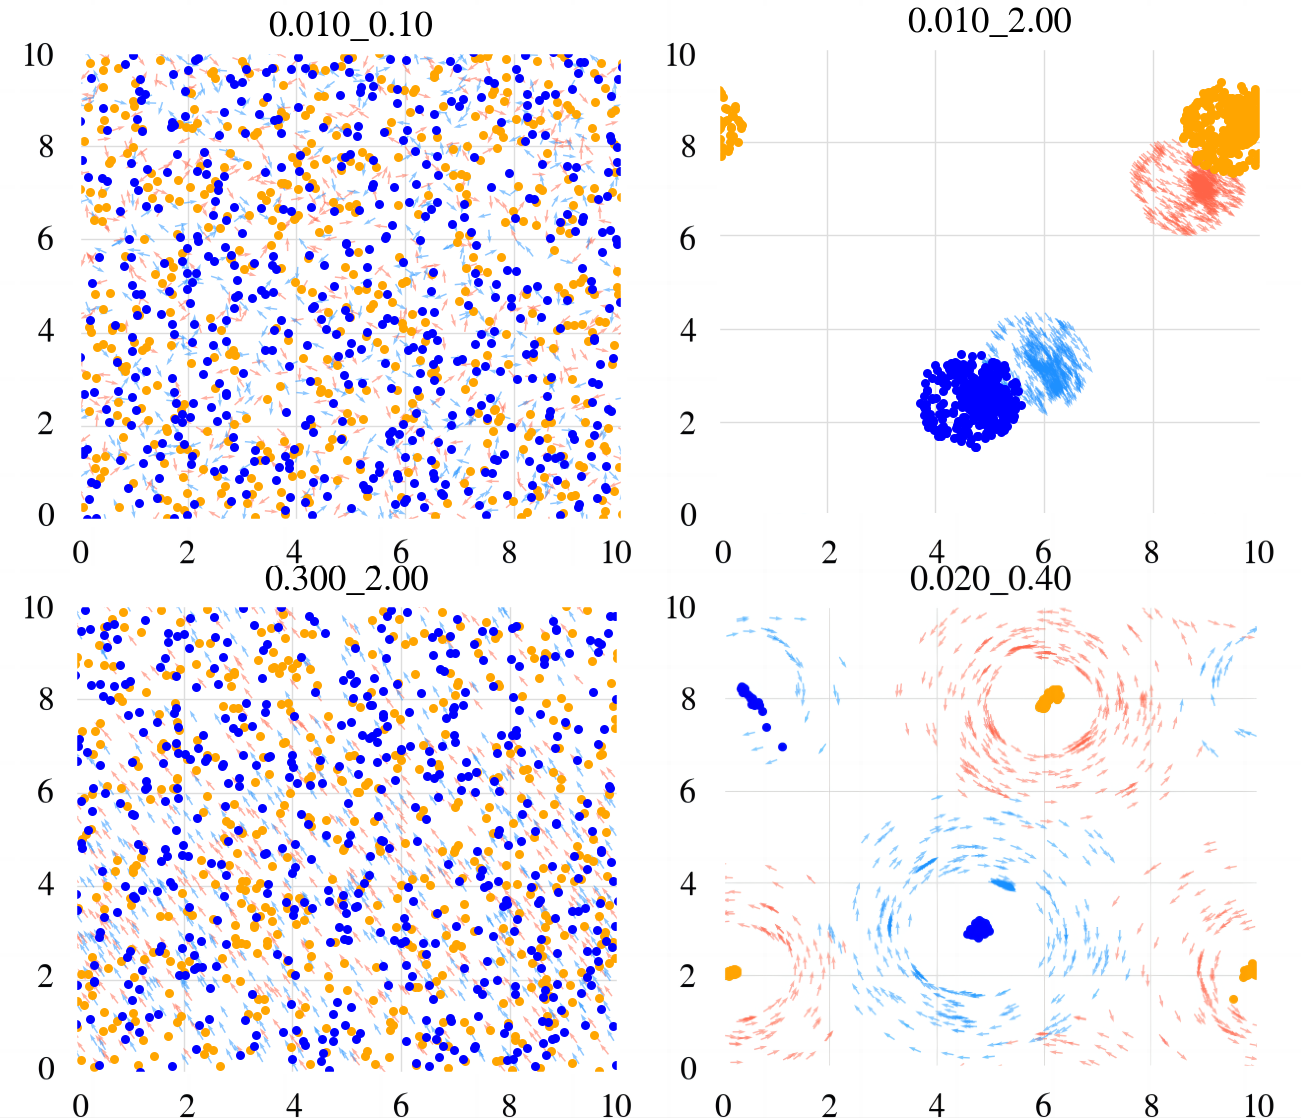
\includegraphics[width=0.7\textwidth]{./figs/centorsBigGraph_sub.png}
	\vspace{-0.2cm}
	\caption{旋转中心求解结果示例}
	\label{fig:fig232.2}
\end{figure}

上图中,带有箭头的半透明色点表示粒子,光滑实心色点表示粒子的旋转中心,其中,橙色点为正手性粒子(半透明红色箭头)的旋转中心,蓝色点为负手性粒子(半透明蓝色箭头)的旋转中心. 从图中可以看出,形成清晰的环态后,环上粒子的旋转中心较为集中,说明同一环上粒子的运动规律较为接近,且近似圆周运动.



\subsubsection{基于调整耦合距离的聚类算法}\label{clustering}

考虑到粒子在形成环态或集群态时,会形成多个环或集群,因此可以对粒子进行聚类从而计算各环或群的局部序参量. 由于环在欧氏空间中的分布较为特殊(中空,环与环相邻),因此改为对粒子的旋转中心进行聚类. 此外,周期性边界条件会导致粒子的旋转中心跨边界,这里采样式\ref{eq:eq1}对旋转中心坐标进行调整.

\begin{algorithm}
	\SetKw{in}{in}
	\SetKwData{Left}{left}\SetKwData{This}{this}\SetKwData{Up}{up}
	\SetKwFunction{Union}{Union}\SetKwFunction{FindCompress}{FindCompress}
	\SetKwInOut{Input}{input}\SetKwInOut{Output}{output}

	\BlankLine
	\KwData{A set $S=\left\{(\bar{x}_i, \bar{y}_i)\right\}$ of particles' circular center coordinates}
	\KwIn{cluster distance $d_{th}$}
	\KwResult{A cluster set $C=\left\{
		\left\{ 1 \right\}
	 \right\}$}
	% \BlankLine
	\emph{$C$ $\leftarrow$ $\left\{(\bar{x}_1, \bar{y}_1)\right\}$}\;
	\For{$i\leftarrow 2$ \KwTo $N$}{\label{forins}
		\For{class set $C_k$ \in $C$}{
			\For{$j$ \in $C_k$}{
				\If(\tcp*[f]{belong to $C_k$}){$\bar{d}_{ij} < d_{th}$}{
					$C_j \leftarrow C_j \cup \left\{i\right\}$\;
					go to line \ref{forins}\;
				}
			}
		}
		$C \leftarrow C \cup \left\{\left\{i\right\}\right\}$; \tcp*[f]{create new class}
	}
	\caption{Clustering algorithm based on adjusted distance}\label{algo_disjdecomp}
\end{algorithm}\DecMargin{1em}

取$d_{th}=1, \lambda=0.02, d_0=0.4, random seed=80$并对模型终态执行算法,可得到如下图\ref{fig:fig233.1}所示的聚类结果. 对比左侧子图与右侧子图,可以发现,算法可以较好地将多个环分开.

\begin{figure}[H]
	\centering
	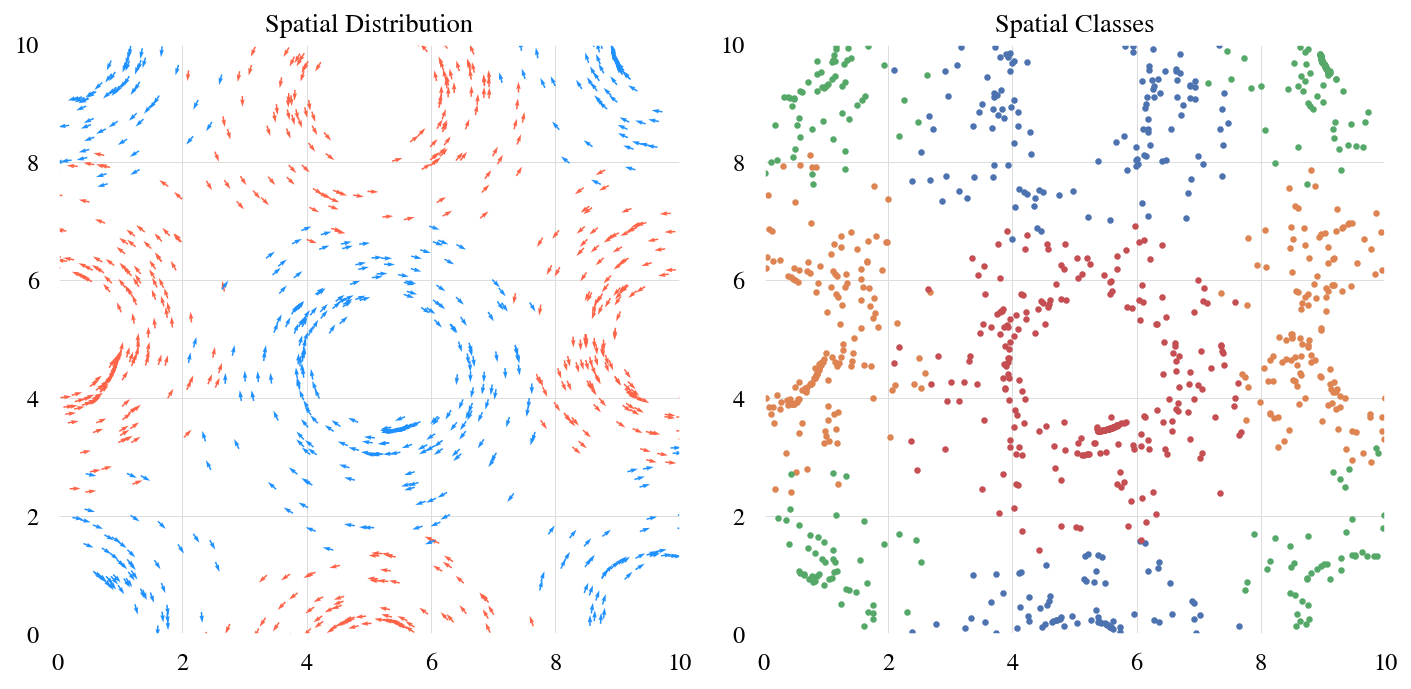
\includegraphics[width=0.9\textwidth]{./figs/ClusteringResult.png}
	\vspace{-0.4cm}
	\caption{聚类结果 ($d_{th}=1, \lambda=0.02, d_0=0.4, random seed=80$)}
	\label{fig:fig233.1}
\end{figure}

\subsubsection{序参量的定义与计算}

为了评估截面序参量对相图的刻画能力,这里根据终态的拓扑结构绘制了主观划分的相图,以提供对比,如下图\ref{fig:fig234.1}所示. 从左至右,从上至下,分别为无序态、环态、集群态、快速同步态. 图\ref{fig:fig232.2}中的四种状态分别对应图\ref{fig:fig234.1}中的四个区域,对比观察可以发现,环态与集群态在空间上的聚集程度较高,而无序态与快速同步态在空间上分布较为均匀,聚集程度低; 此外,集群态与快速同步态在相位(速度方向)上的同步程度较高,而环态与无序态较低.

\begin{figure}[H]
	\centering
	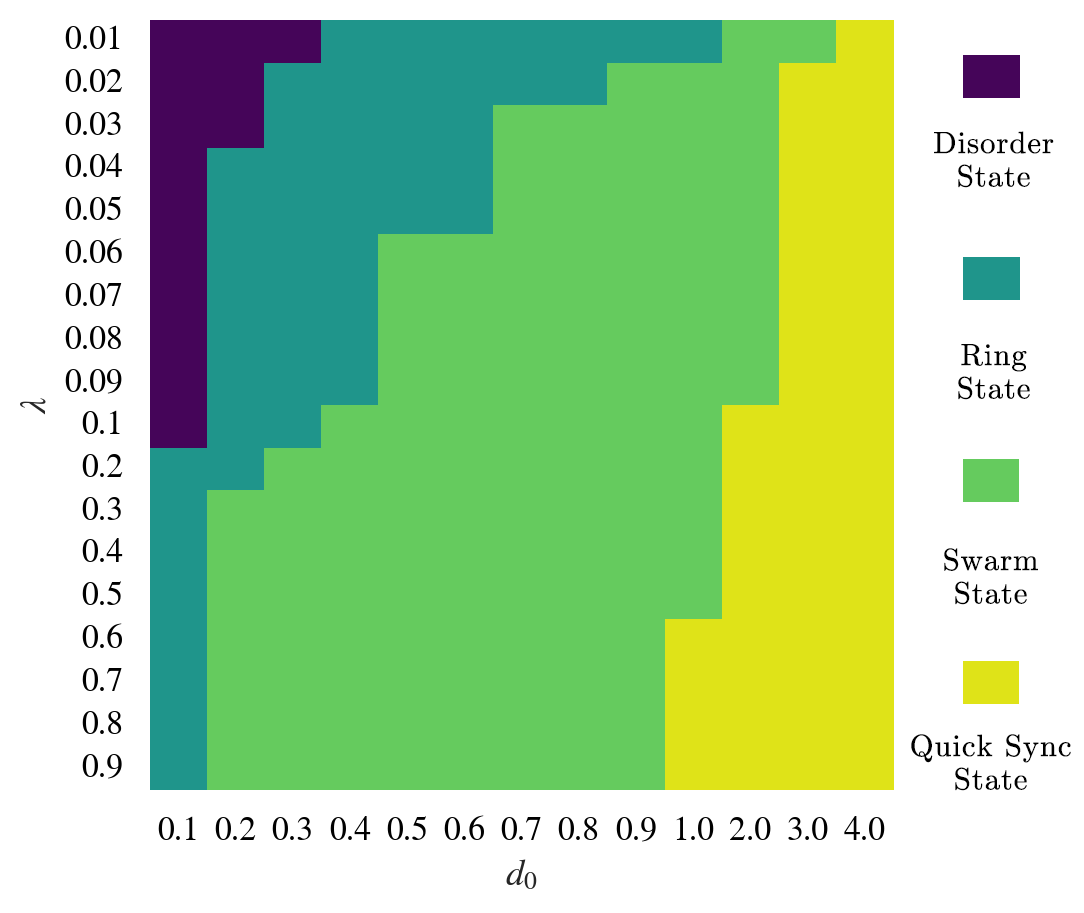
\includegraphics[width=0.5\textwidth]{./figs/subjectiveOp.png}
	\vspace{-0.5cm}
	\caption{主观划分相图}
	\label{fig:fig234.1}
\end{figure}
\vspace{-0.5cm}

\noindent\textbf{相位(速度方向)同步率(截面序参量)}

$$
r e^{i\psi}=\frac{1}{N}\sum_{j=1}^{N}{e^{i\theta _j}}
$$

\begin{figure}[H]
	\centering
	\begin{subfigure}[b]{0.49\textwidth}
		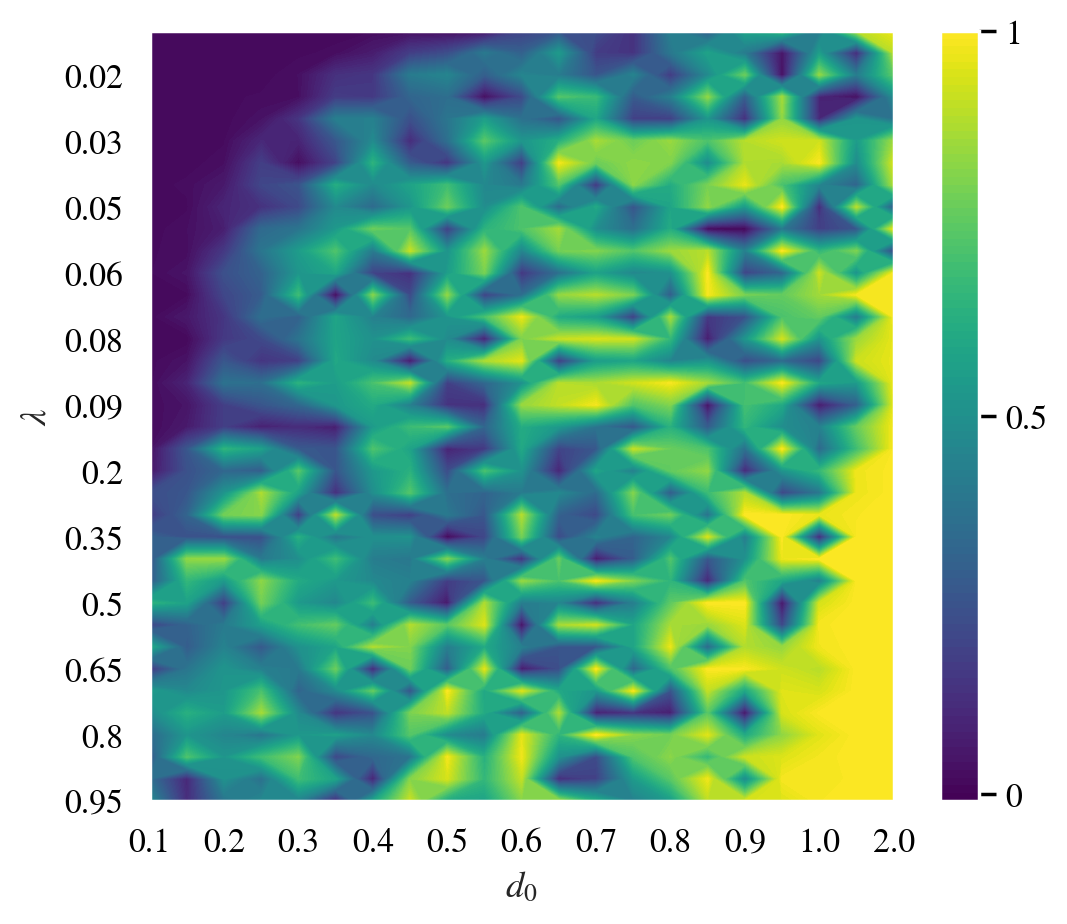
\includegraphics[width=\textwidth]{./figs/phaseSyncOp.png}
		\vspace{-1cm}
		\caption{计算结果}
	\end{subfigure}
	% \hfill
	\begin{subfigure}[b]{0.49\textwidth}
		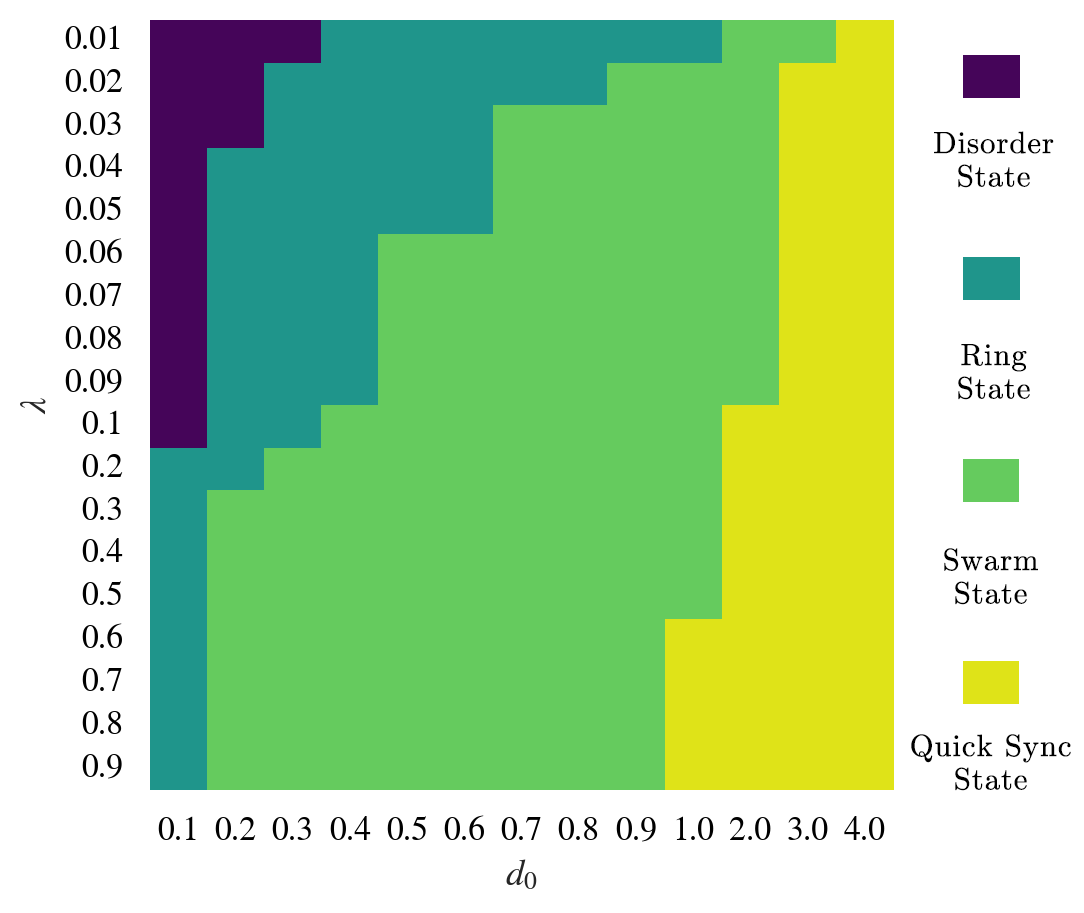
\includegraphics[width=\textwidth]{./figs/subjectiveOp.png}
		\vspace{-1cm}
		\caption{主观划分相图}
	\end{subfigure}
	\vspace{-0.5cm}
	\caption{相位(速度方向)同步率}
	\label{fig:fig234c.1}
\end{figure}

\vspace{-0.5cm}
由于部分集群态存在分裂现象,因此某些集群态的全局相位同步程度较低,导致该序参量过渡不均匀,不易区分环态与集群态. 针对这个问题的改进见\ref{fig:fig234c.5}和\ref{fig:fig234c.6}

% 观察图\ref{fig:fig234.2},可以发现,该序参量可以较好地将空间当中的聚集情况反映出来.左上角与右下角深色区域的粒子在空间上没有形成聚集,而中间部分的粒子在空间上形成了聚集.此外,集群态的序参量取值比环态的序参量取值小,这是因为集群态的旋转中心集中度较低,导致与原点距离的标准差更小.

\newpage
\noindent\textbf{旋转中心空间聚集程度1(截面序参量)}

这里以粒子旋转中心间的距离来刻画中心的空间聚集程度,考虑到周期性边界条件,这里采用式\ref{eq:eq1}对旋转中心坐标进行调整,然后计算所有粒子旋转中心间距离的算数平均,即

$$
\frac{1}{N}\sum_{i=1}^N{\left( \frac{1}{N}\sum_{j=1}^N{\bar{d}_{ij}} \right)}
$$

其中,$\bar{d}_{ij}$为调整后的粒子$i$与粒子$j$的旋转中心距离.

\begin{figure}[H]
	\centering
	\begin{subfigure}[b]{0.49\textwidth}
		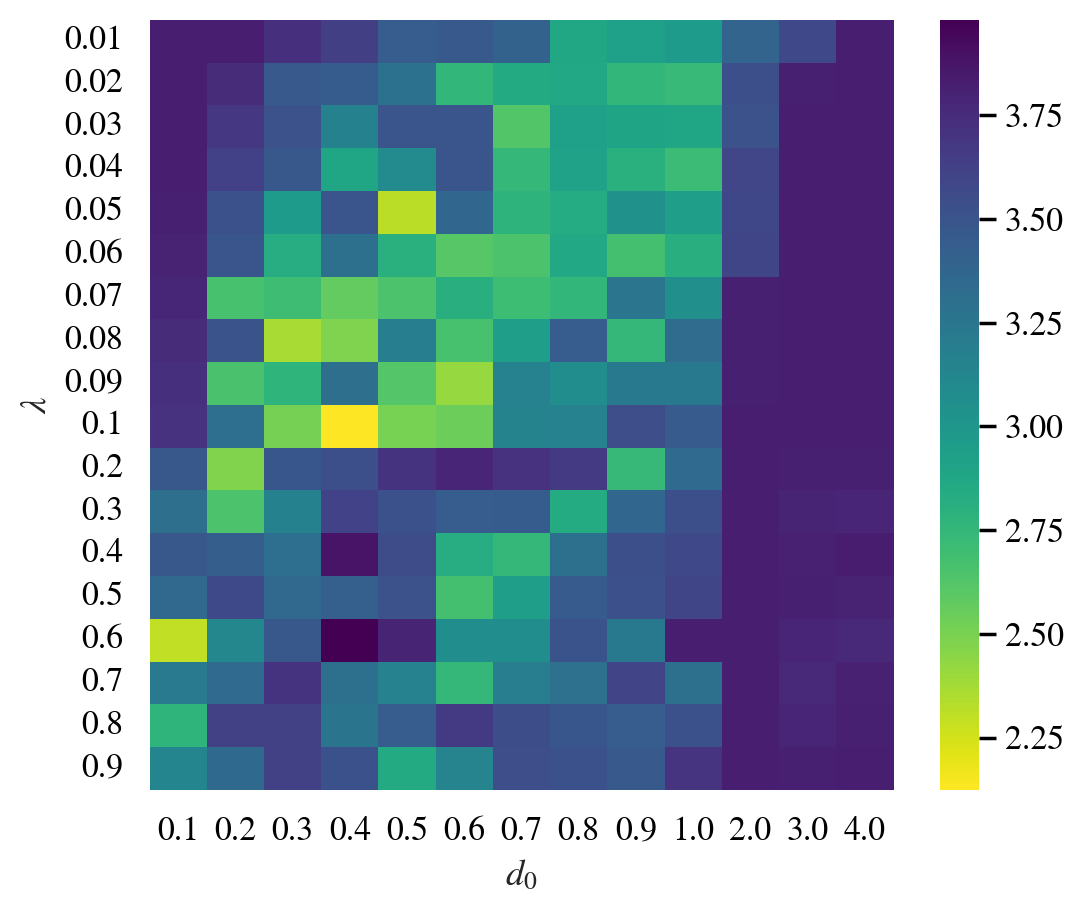
\includegraphics[width=\textwidth]{./figs/centerAggOp1.png}
		\vspace{-1cm}
		\caption{计算结果}
	\end{subfigure}
	% \hfill
	\begin{subfigure}[b]{0.49\textwidth}
		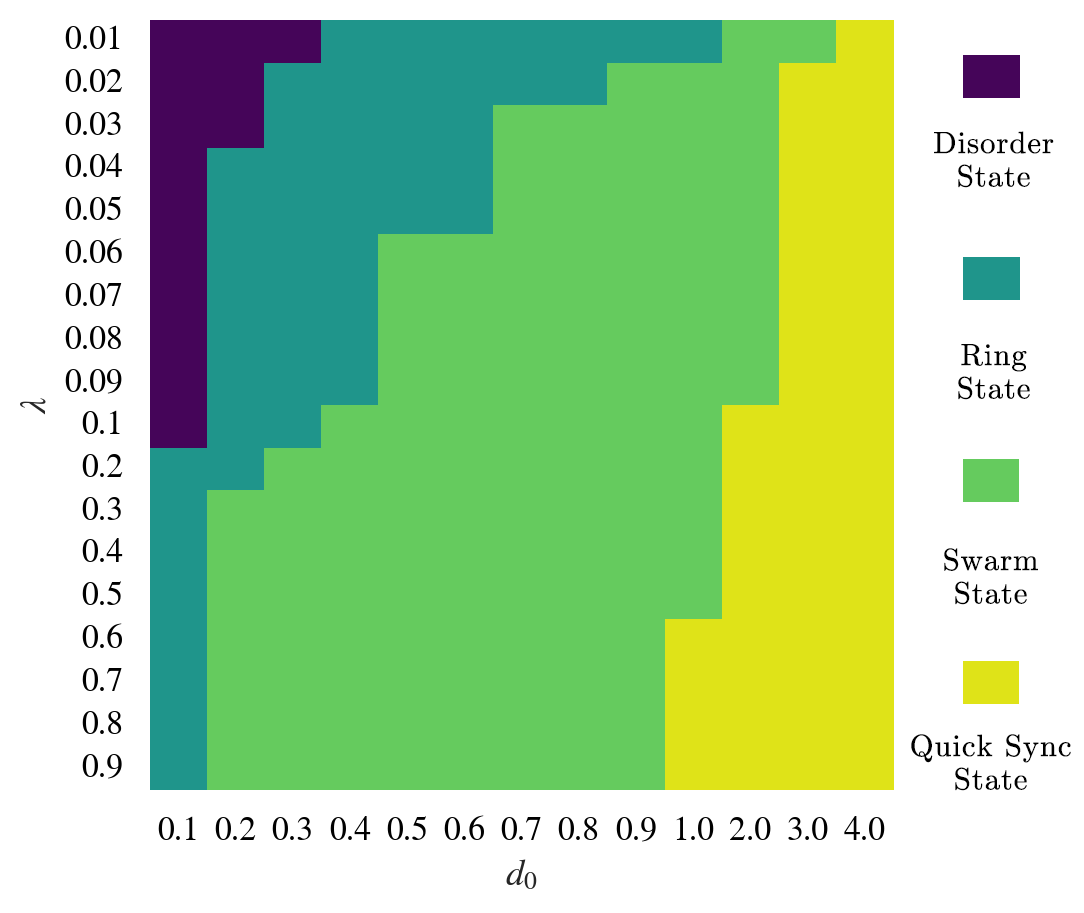
\includegraphics[width=\textwidth]{./figs/subjectiveOp.png}
		\vspace{-1cm}
		\caption{主观划分相图}
	\end{subfigure}
	\vspace{-0.5cm}
	\caption{旋转中心空间聚集程度1}
	\vspace{-0.5cm}
	\label{fig:fig234c.3}
\end{figure}

\noindent\textbf{旋转中心空间聚集程度2(截面序参量)}

$$
\frac{1}{N}\sum_{i=1}^N{\left| \frac{\sum\nolimits_{j=1}^N{\mathbf{C}_i-\bar{\mathbf{C}}_j}}{N} \right|}
$$

其中,$\bar{\mathbf{C}}_j$为第$j$个粒子旋转中心以第$i$个粒子旋转中心为基准,根据方法\ref{positionAdj}调整后的坐标.

\begin{figure}[H]
	\centering
	\begin{subfigure}[b]{0.49\textwidth}
		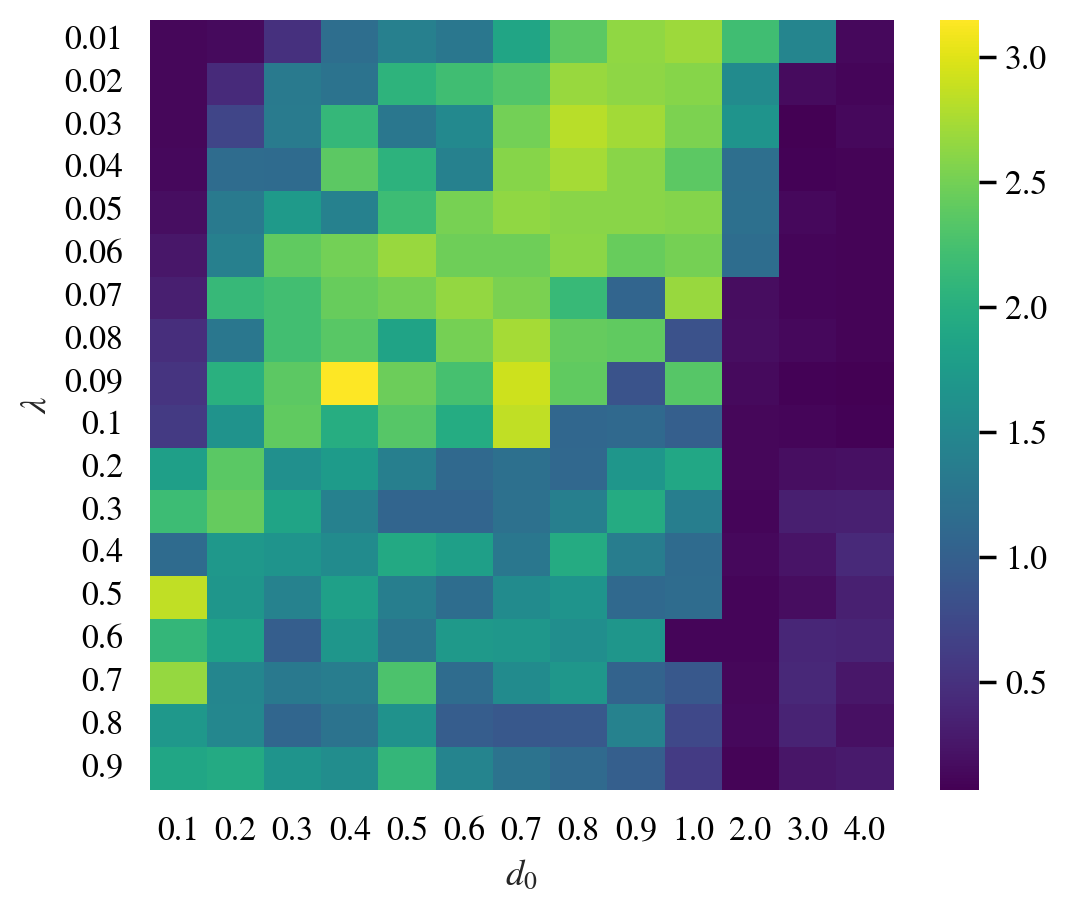
\includegraphics[width=\textwidth]{./figs/centerAggOp2.png}
		\vspace{-1cm}
		\caption{计算结果}
	\end{subfigure}
	% \hfill
	\begin{subfigure}[b]{0.49\textwidth}
		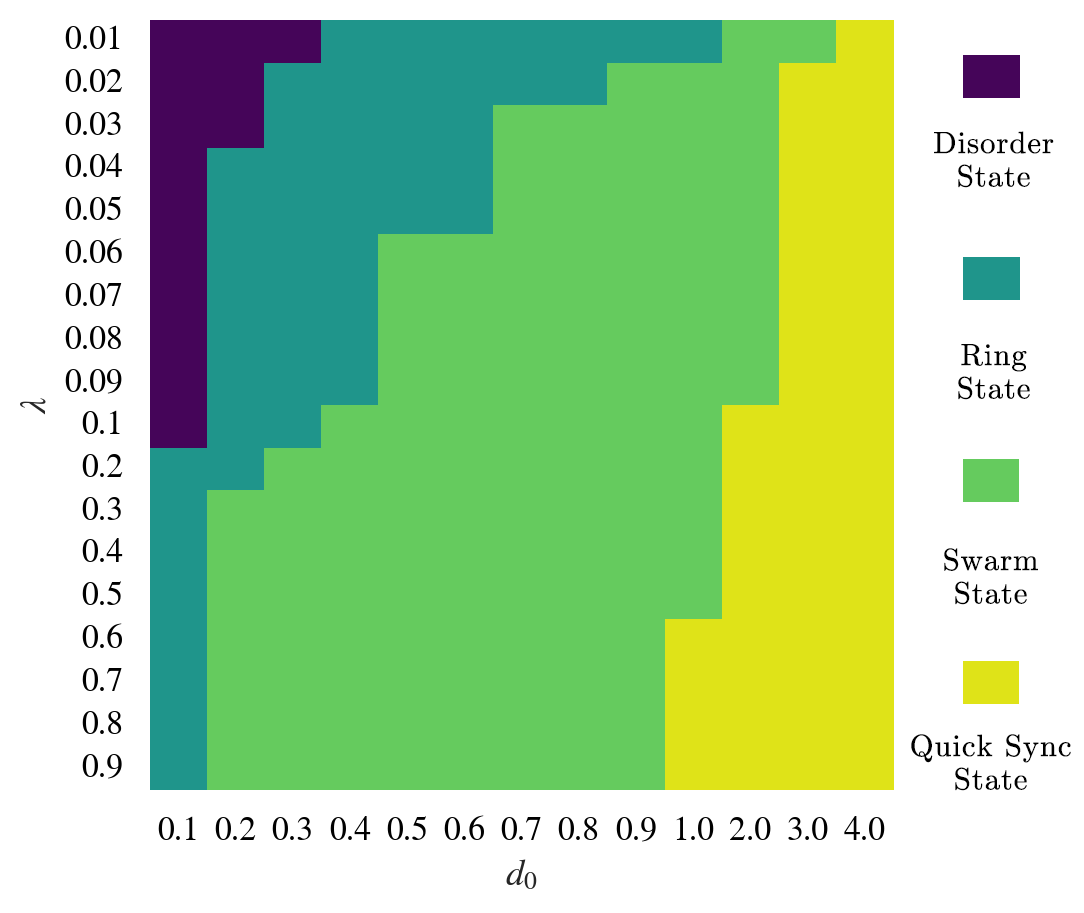
\includegraphics[width=\textwidth]{./figs/subjectiveOp.png}
		\vspace{-1cm}
		\caption{主观划分相图}
	\end{subfigure}
	\vspace{-0.5cm}
	\caption{旋转中心空间聚集程度2}
	\label{fig:fig234c.4}
\end{figure}

\newpage
\noindent\textbf{聚类平均相位同步程度(截面序参量)}

这里基于方法\ref{clustering}($d_{th}=1$)对粒子旋转中心进行聚类,然后计算每一类(粒子数不足5个的分类剔除)中粒子的相位同步程度,最后取所有类的相位同步程度的算数平均,即

$$
\frac{1}{N_{class}}\sum_{k=1}^{N_{class}}{\left( \frac{1}{N_k}\sum_{i\in C_k}{\left| r e^{i\psi} \right|} \right)}
$$

\vspace{-0.5cm}
\begin{figure}[H]
	\centering
	\begin{subfigure}[b]{0.49\textwidth}
		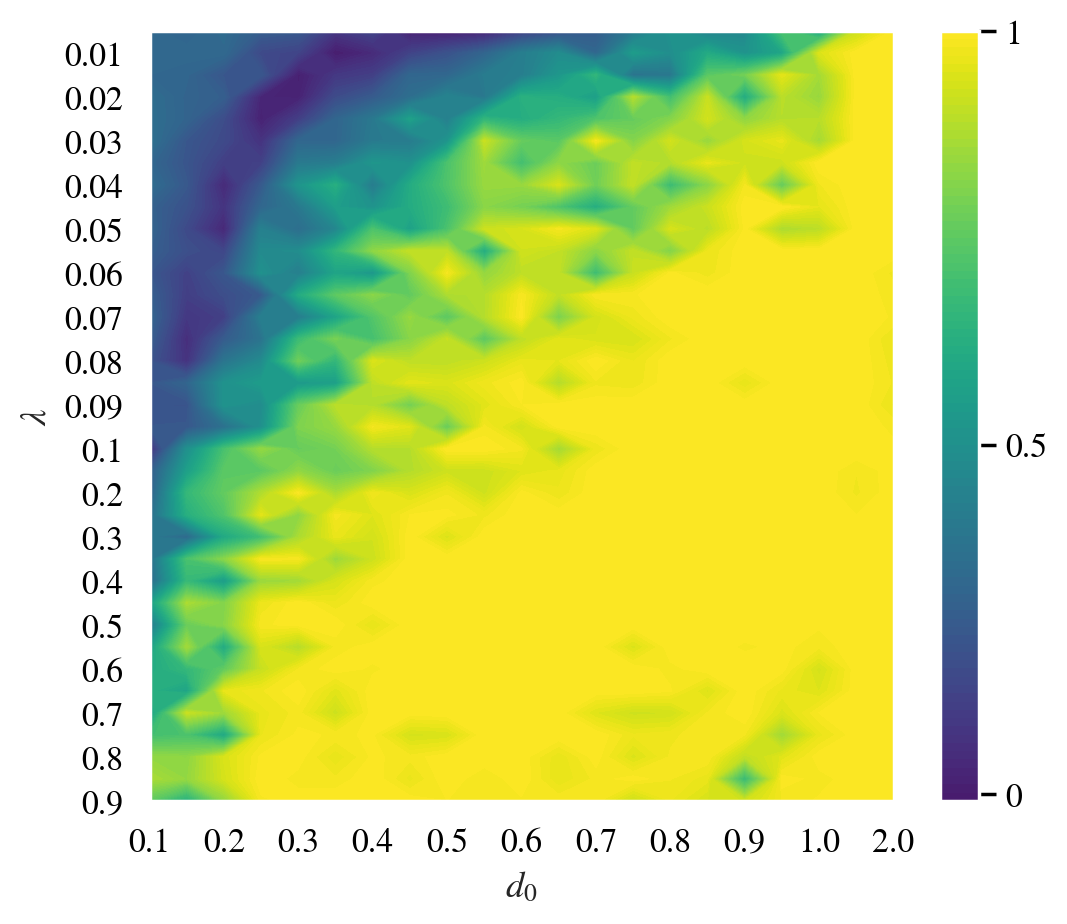
\includegraphics[width=\textwidth]{./figs/clusteringPhaseSync.png}
		\vspace{-1cm}
		\caption{计算结果}
	\end{subfigure}
	% \hfill
	\begin{subfigure}[b]{0.49\textwidth}
		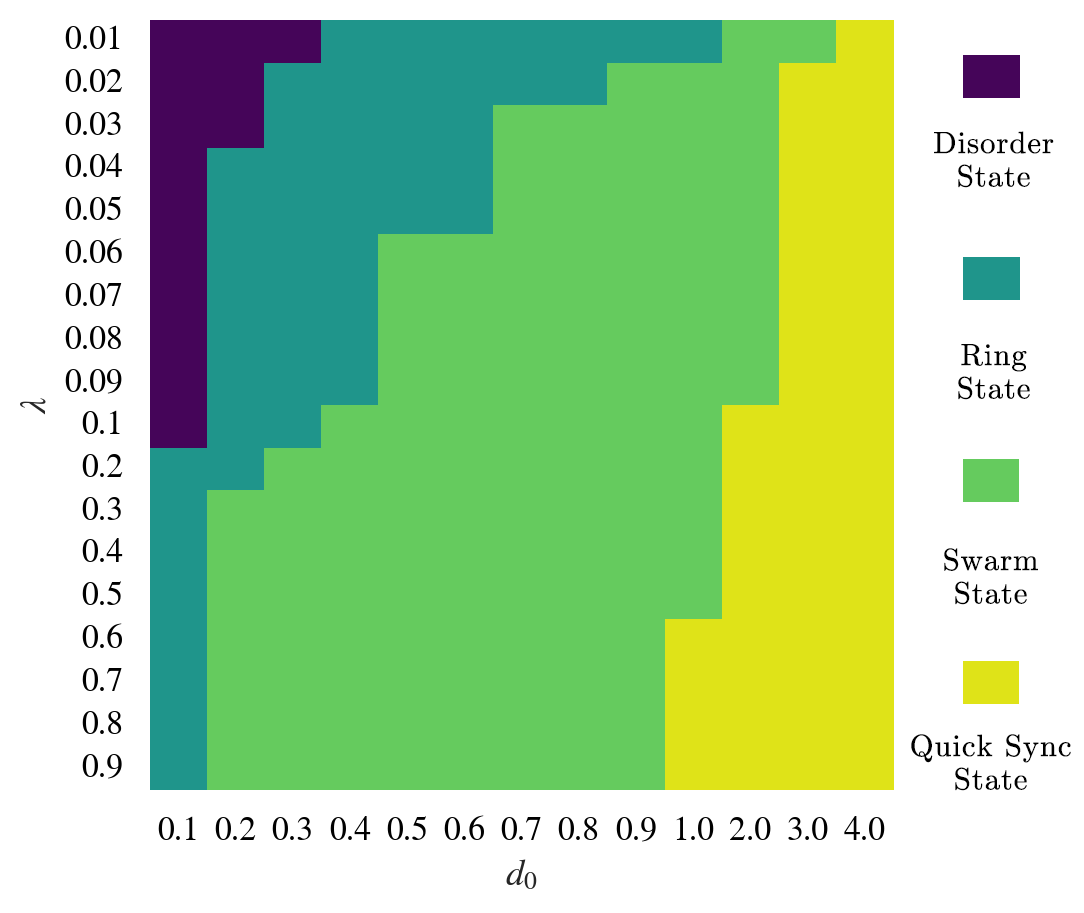
\includegraphics[width=\textwidth]{./figs/subjectiveOp.png}
		\vspace{-1cm}
		\caption{主观划分相图}
	\end{subfigure}
	\vspace{-0.5cm}
	\caption{聚类平均相位同步程度}
	\label{fig:fig234c.5}
\end{figure}

\vspace{-0.5cm}
对比图\ref{fig:fig234c.1}可以发现,图\ref{fig:fig234c.5}能够更好地刻画环态与集群态的相位同步程度, 从而将它们区分, 但算法\ref{clustering}的计算复杂度较高,且不易区分集群态与快速同步态,因此做出如下改进:

\noindent\textbf{中心距离倒数加权相位同步程度(截面序参量)}

\begin{equation}\label{weightedPhaseSync}
	S = \frac{1}{N}\sum_{i=1}^N{\left| \frac{\sum\nolimits_{j\ne i}^N{e^{i\theta _j/\bar{d}_{ij}}}}{\sum\nolimits_{j\ne i}^N{1/\bar{d}_{ij}}} \right|}
\end{equation}

\vspace{-0.5cm}
\begin{figure}[H]
	\centering
	\begin{subfigure}[b]{0.49\textwidth}
		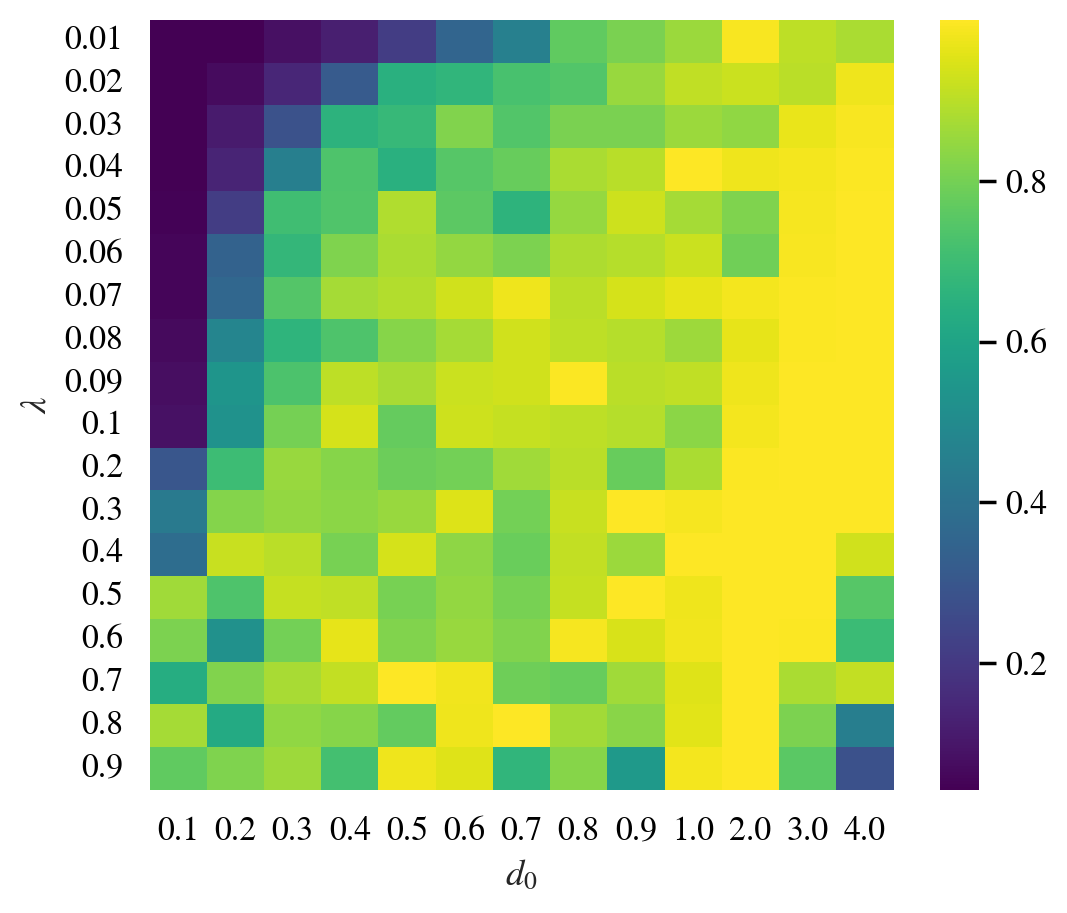
\includegraphics[width=\textwidth]{./figs/weightedPhaseSync.png}
		\vspace{-1cm}
		\caption{计算结果}
		
	\end{subfigure}
	% \hfill
	\begin{subfigure}[b]{0.49\textwidth}
		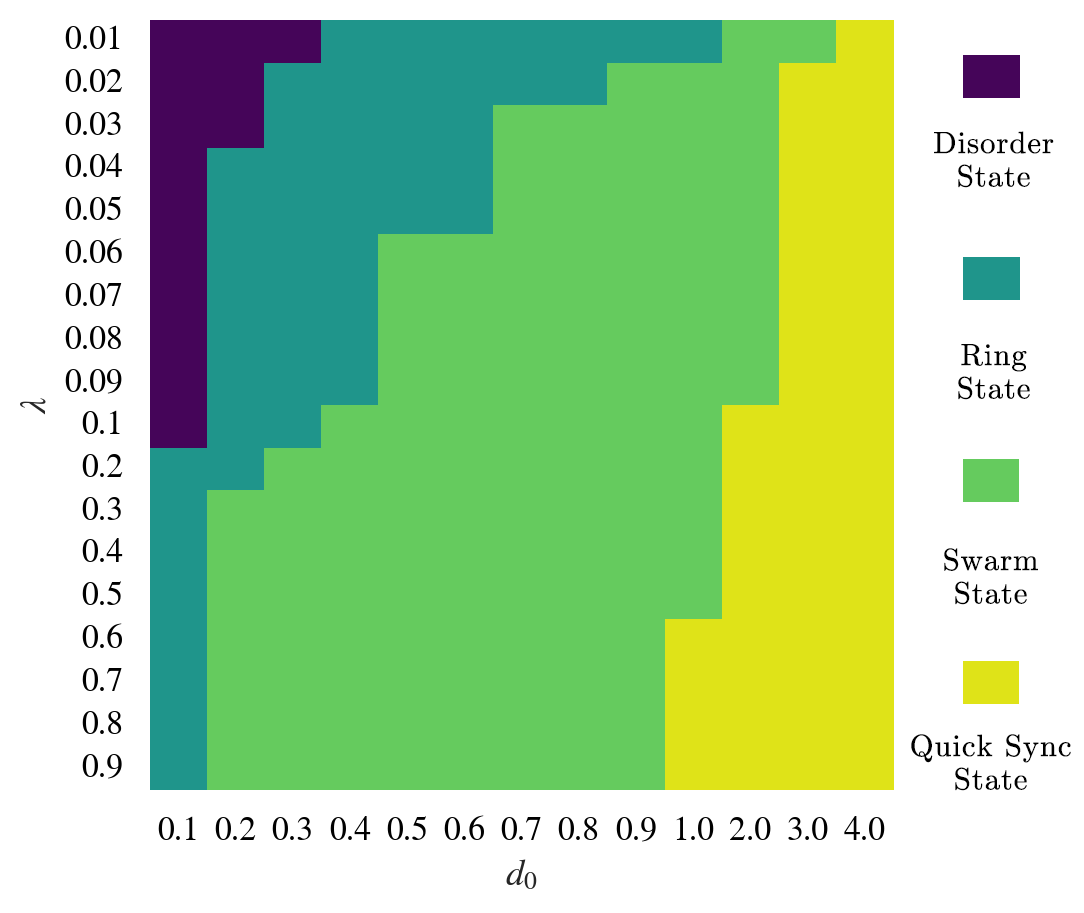
\includegraphics[width=\textwidth]{./figs/subjectiveOp.png}
		\vspace{-1cm}
		\caption{主观划分相图}
	\end{subfigure}
	\vspace{-0.5cm}
	\caption{中心距离倒数加权相位同步程度}
	\label{fig:fig234c.6}
\end{figure}

\vspace{-0.5cm}
对比图\ref{fig:fig234c.5}可以发现两序参量的刻画能力相近,但图\ref{fig:fig234c.6}能够将集群态与快速同步态相区分,与主观划分相图更接近. 此外,式\ref{weightedPhaseSync}的计算复杂度更低.

\newpage
\noindent\textbf{旋转中心空间分布(时序序参量)}

考虑到粒子在二维平面上运动,因此该序参量分为$x$坐标和$y$坐标两个分量,将各粒子旋转中心坐标以散点图形式分别绘制得到图下图像:

\begin{figure}[H]
	\centering
	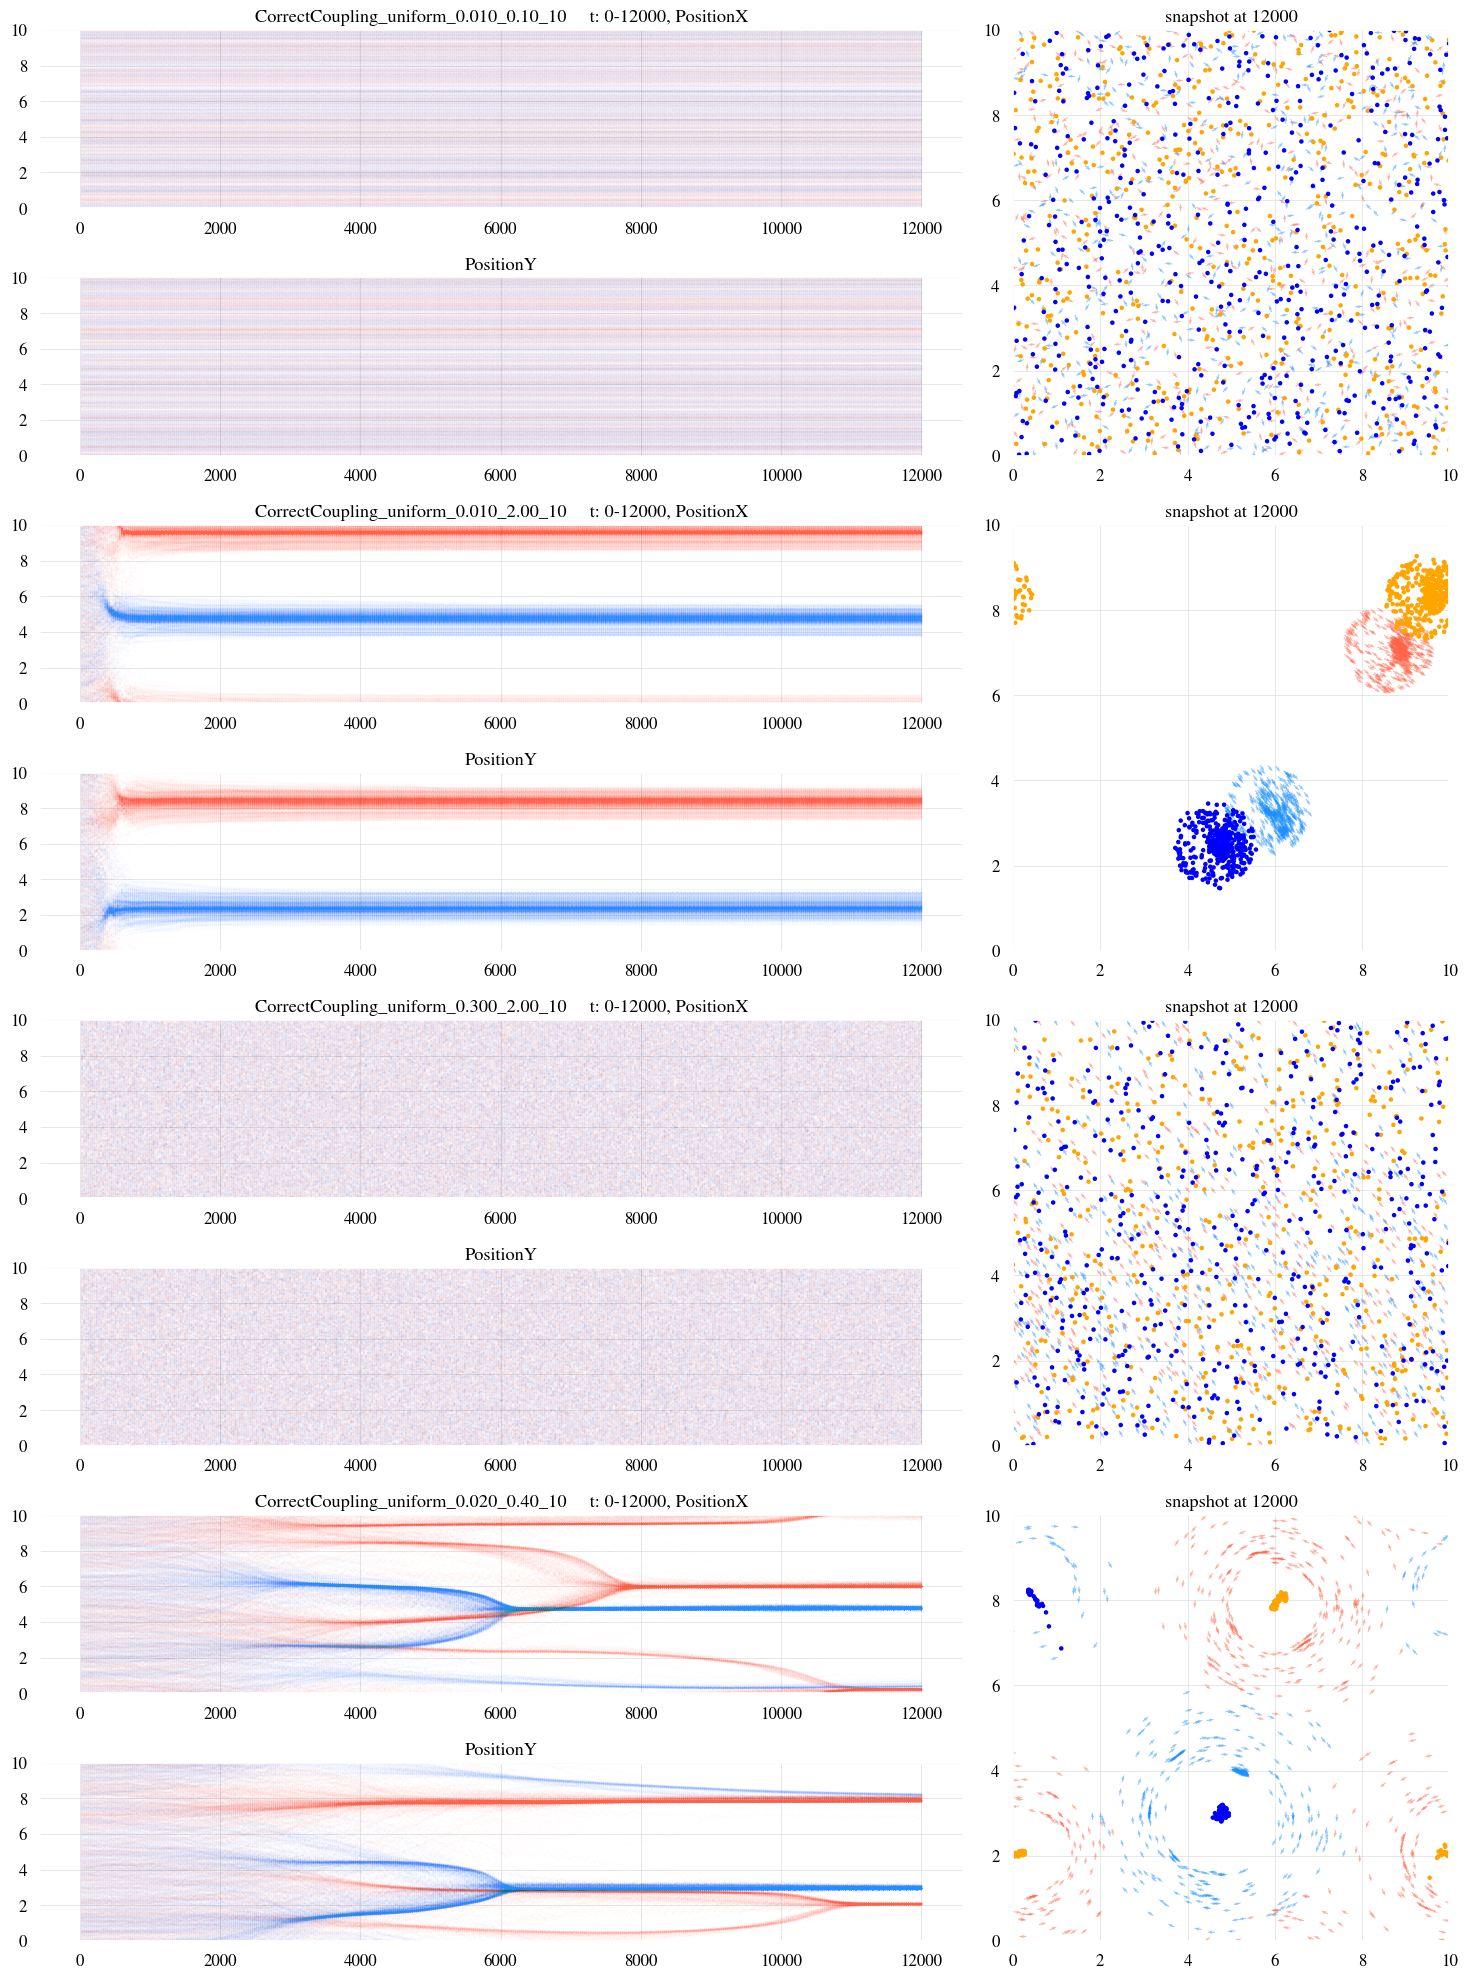
\includegraphics[width=0.9\textwidth]{./figs/totalXY.png}
	\vspace{-0.5cm}
	\caption{旋转中心空间分布}
	\label{fig:fig234t.1}
\end{figure}

\newpage
\noindent\textbf{中心距离倒数加权相位同步程度(各粒子/时序序参量)}

$$
S_i=\left| \frac{\sum\nolimits_{j\ne i}^N{e^{i\theta _j/\bar{d}_{ij}}}}{\sum\nolimits_{j\ne i}^N{1/\bar{d}_{ij}}} \right|
$$

\begin{figure}[H]
	\centering
	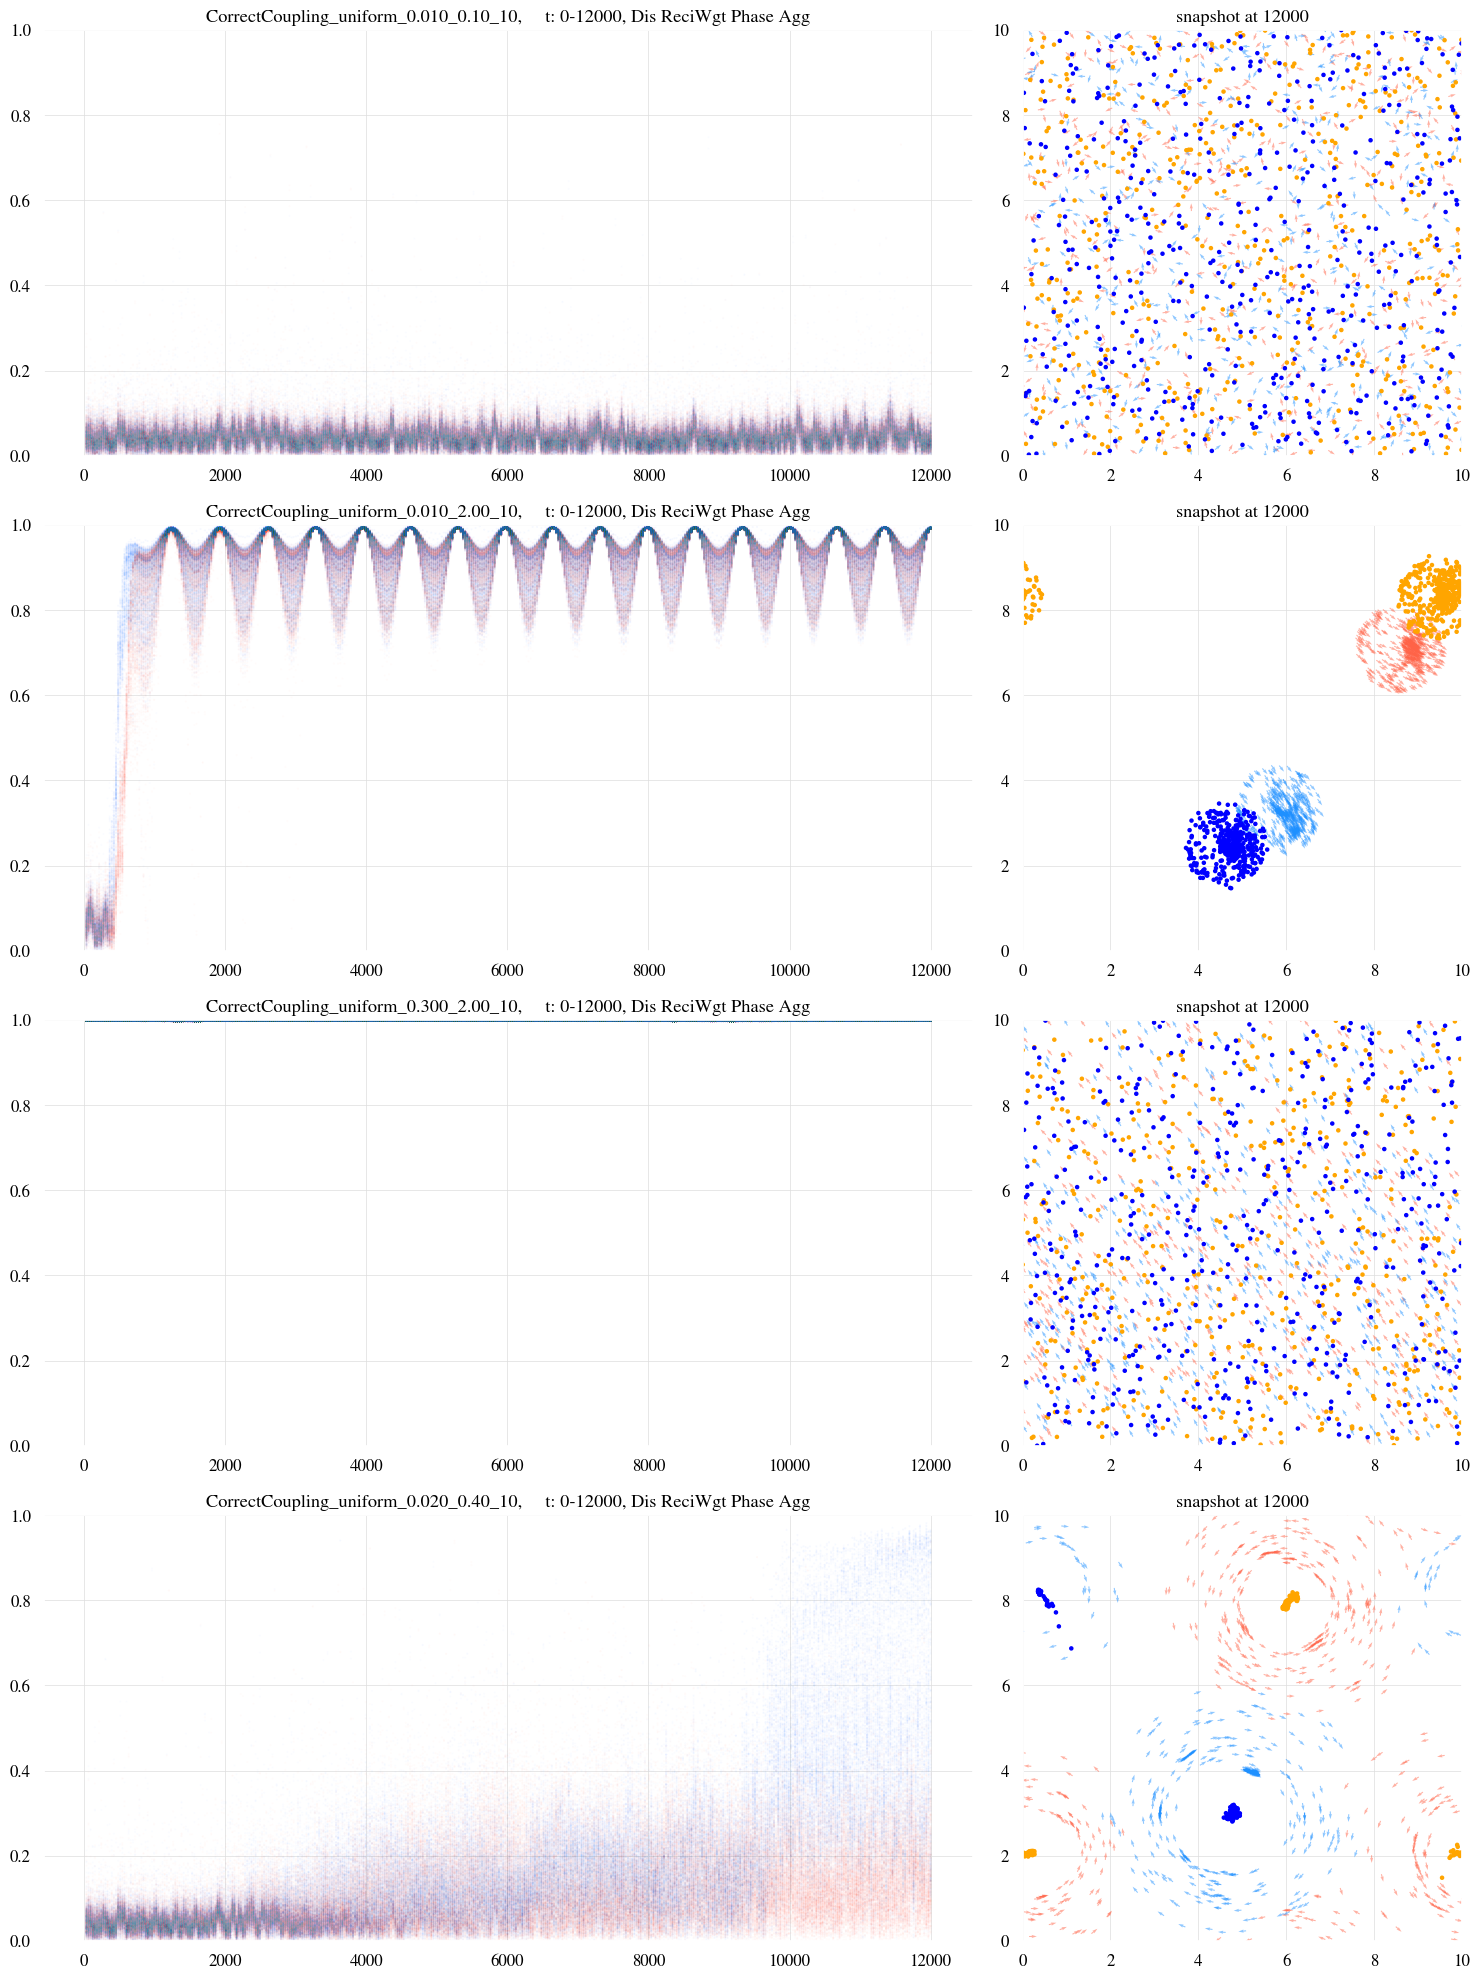
\includegraphics[width=0.9\textwidth]{./figs/weightedPhaseSync_ts.png}
	\vspace{-0.5cm}
	\caption{中心距离倒数加权相位同步程度(各粒子)}
	\label{fig:fig234t.2}
\end{figure}

\newpage
\noindent\textbf{中心距离倒数加权相位同步程度(全局/时序序参量)}

$$
S = \frac{1}{N}\sum_{i=1}^N{\left| \frac{\sum\nolimits_{j\ne i}^N{e^{i\theta _j/\bar{d}_{ij}}}}{\sum\nolimits_{j\ne i}^N{1/\bar{d}_{ij}}} \right|}
$$

\begin{figure}[H]
	\centering
	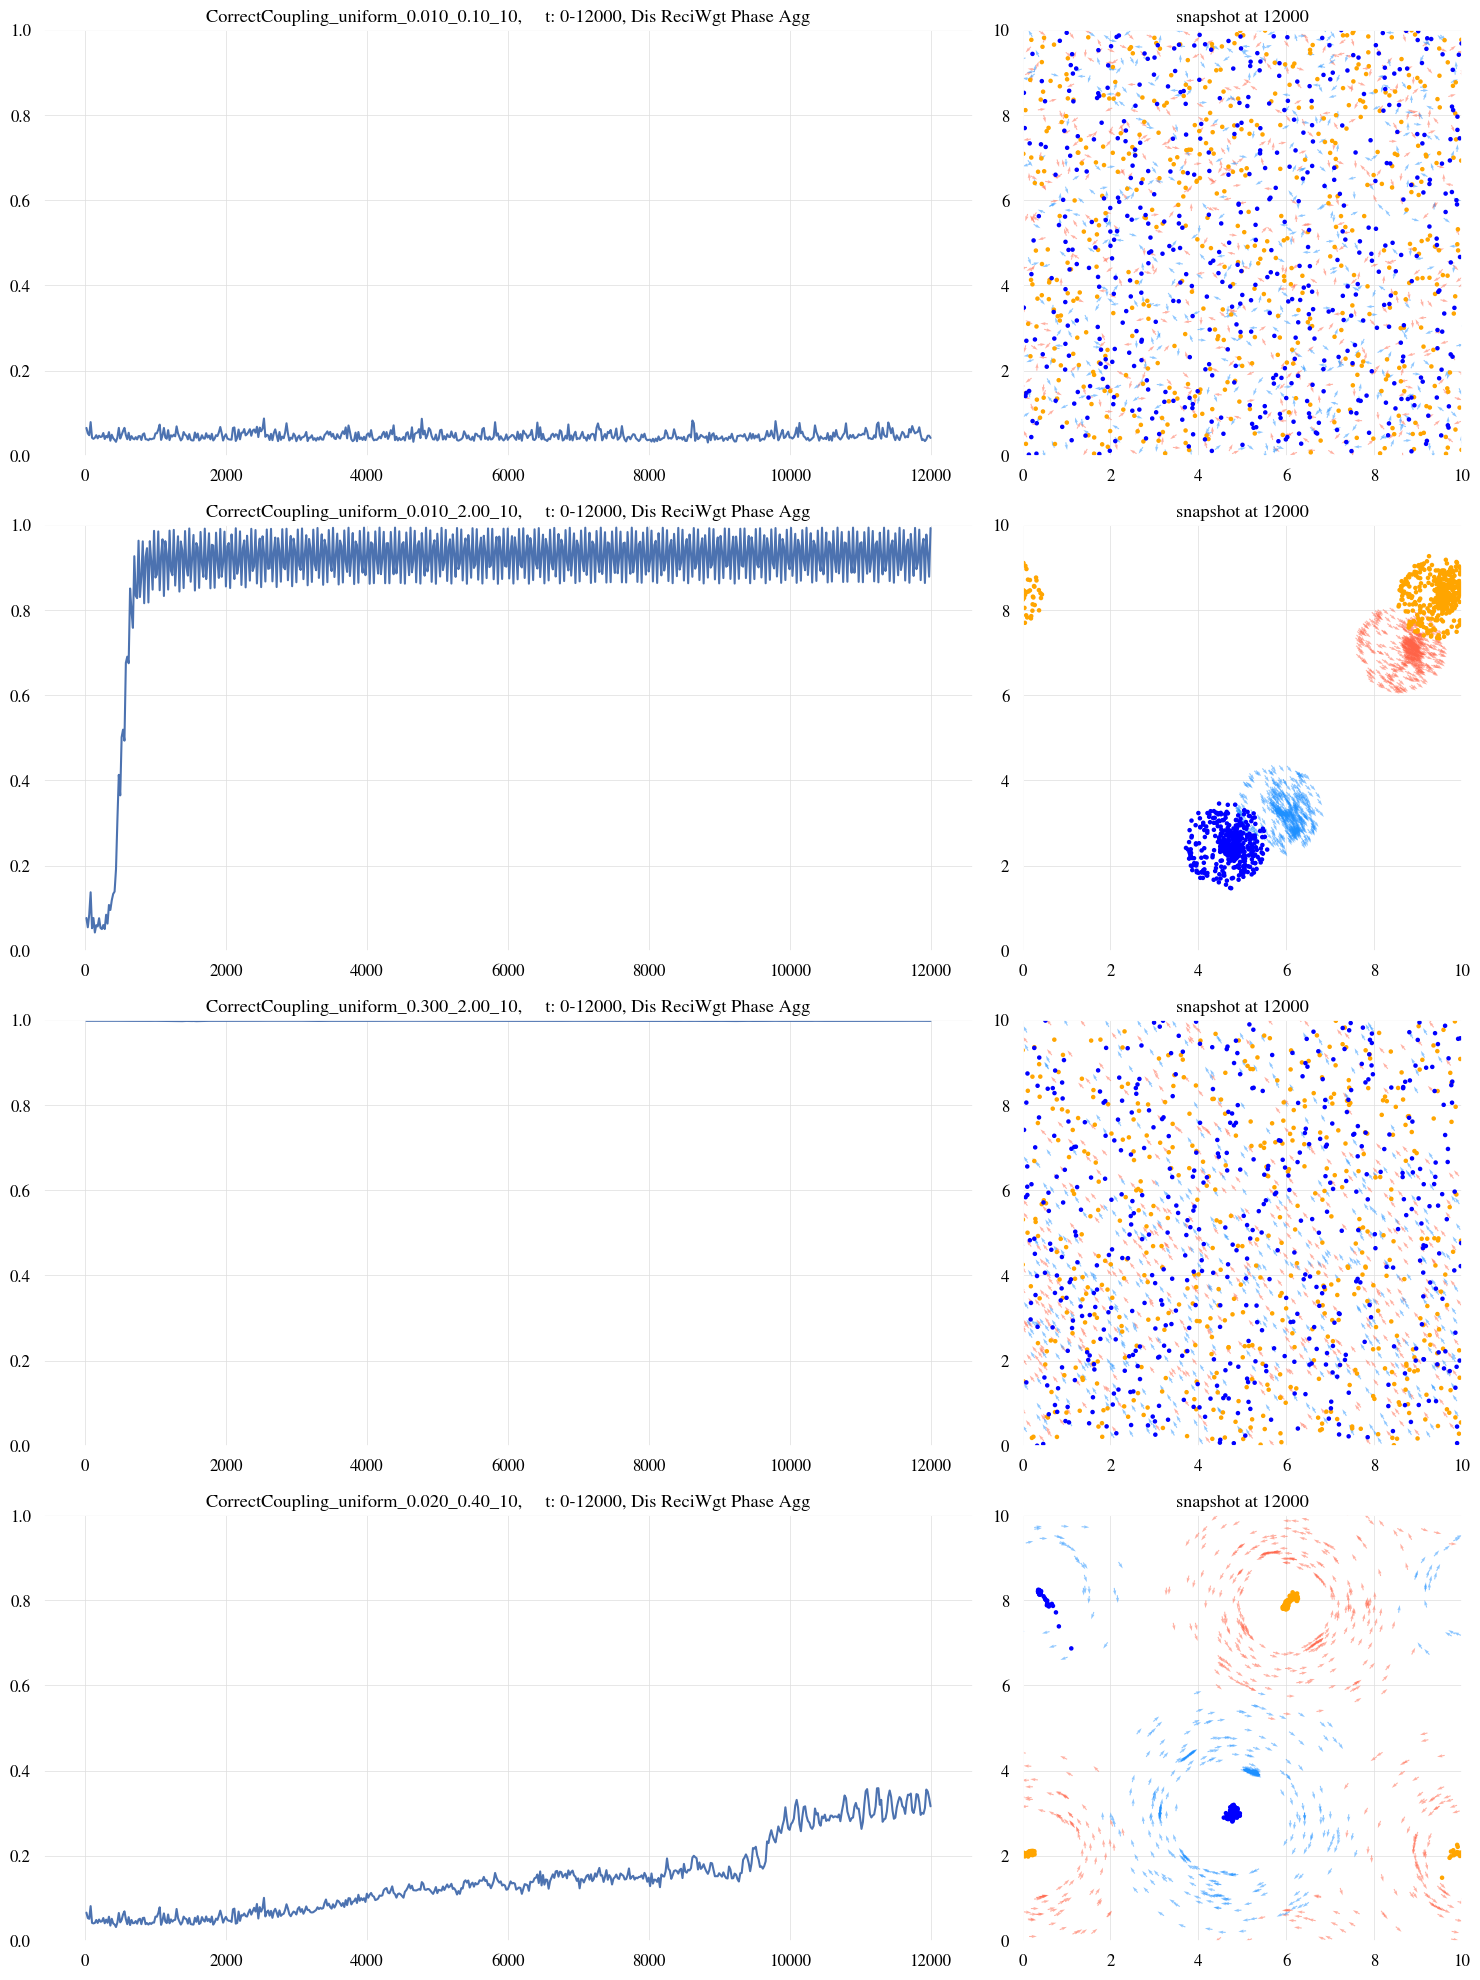
\includegraphics[width=0.9\textwidth]{./figs/weightedPhaseSyncOp_ts.png}
	\vspace{-0.5cm}
	\caption{中心距离倒数加权相位同步程度(全局)}
	\label{fig:fig234t.3}
\end{figure}

\newpage
\noindent\textbf{旋转中心空间聚集程度1(时序序参量)}

\begin{figure}[H]
	\centering
	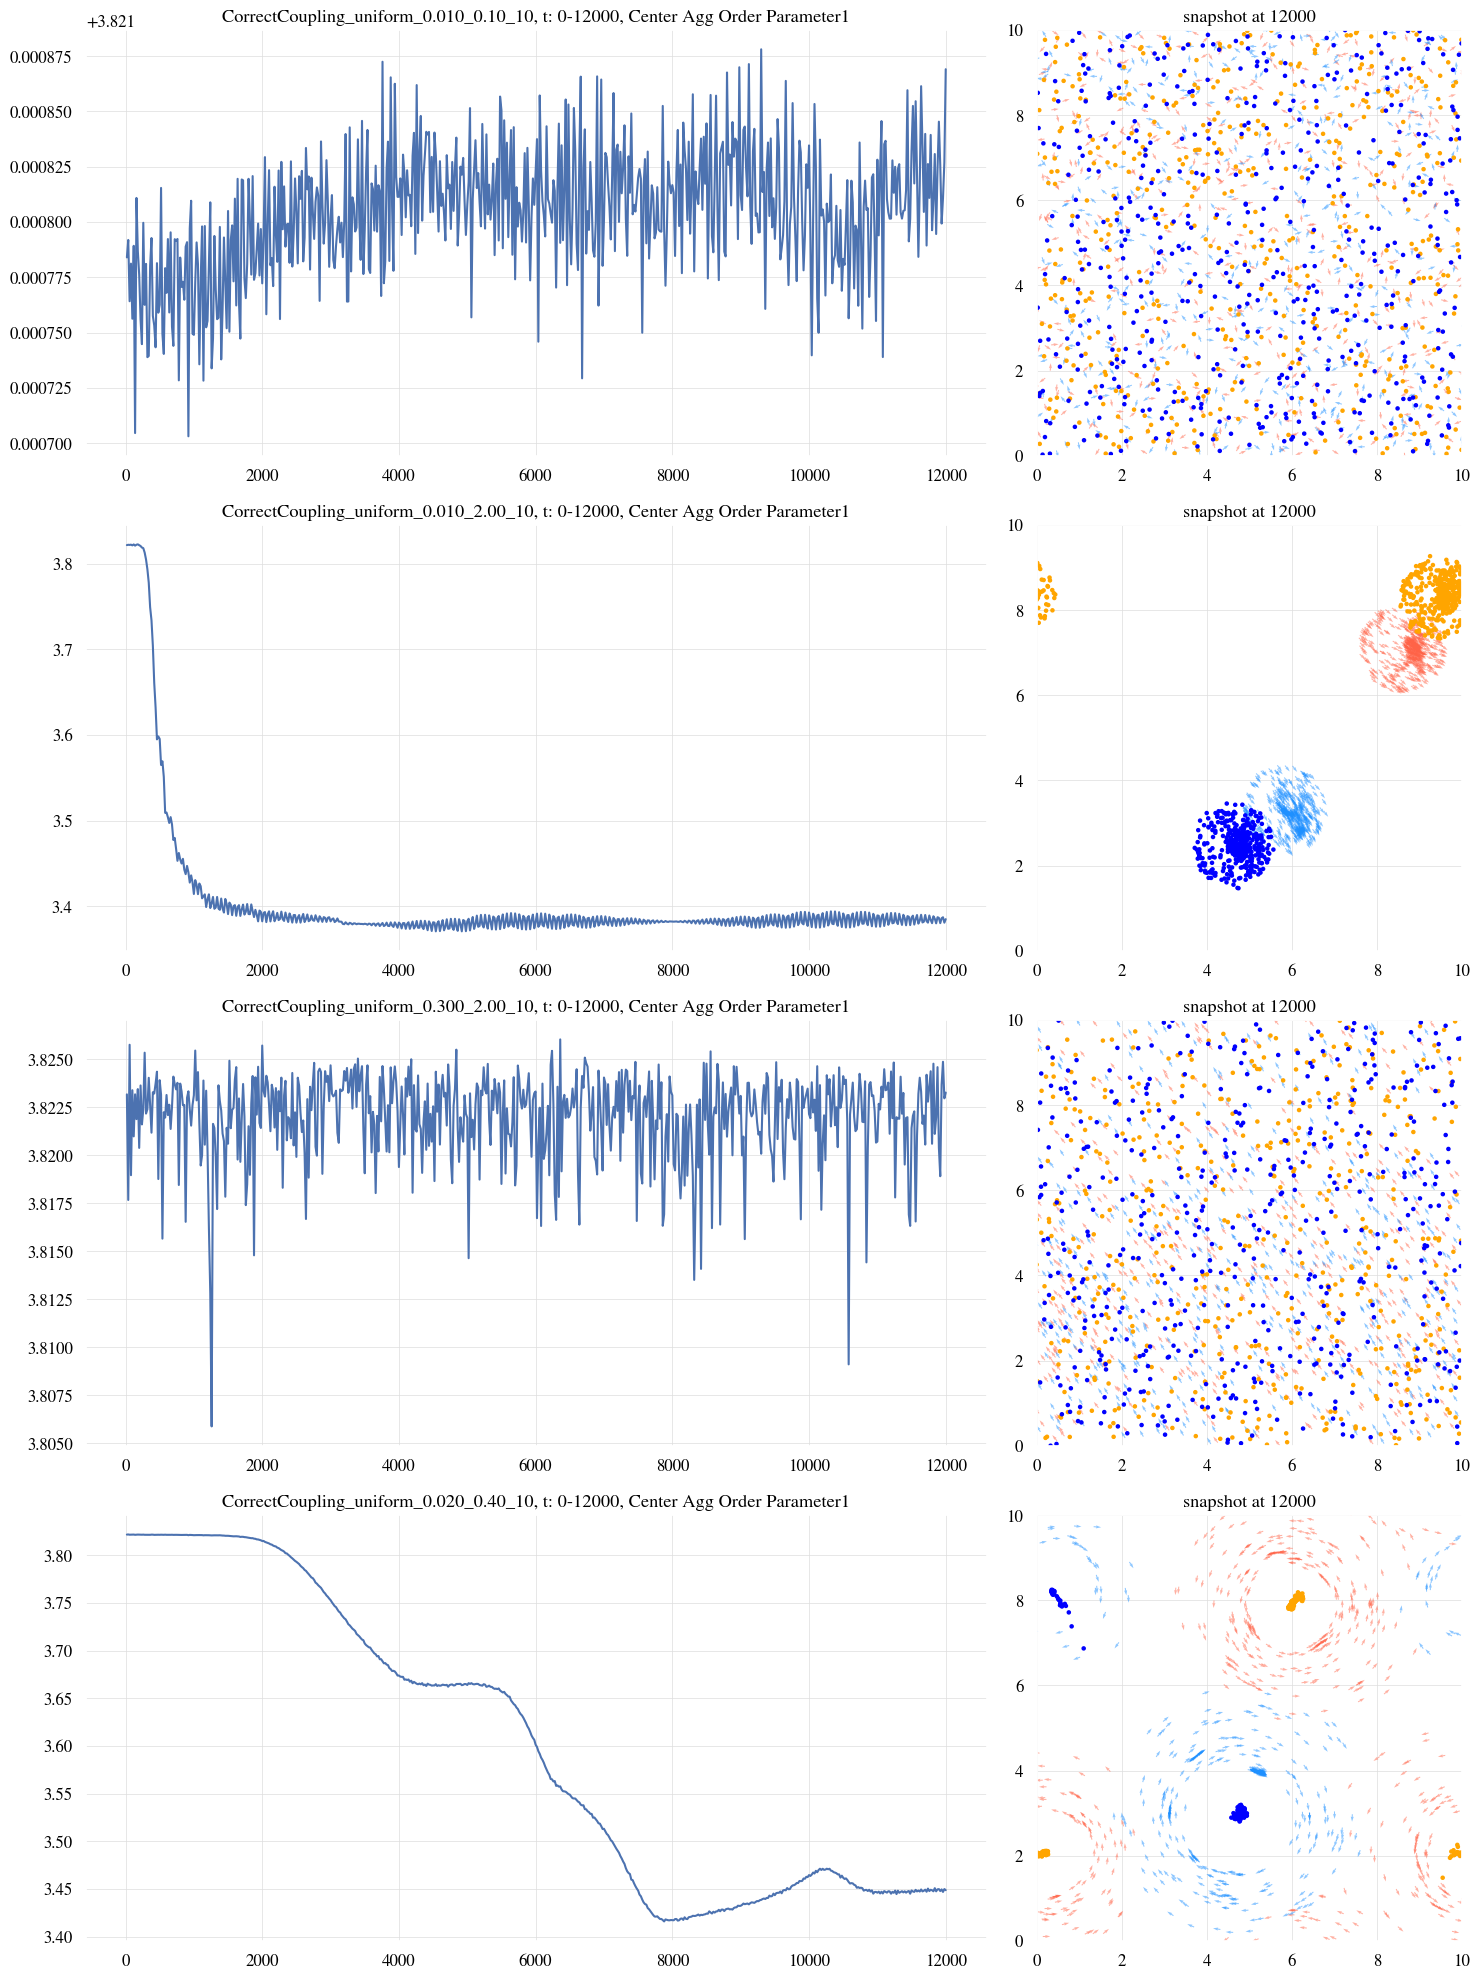
\includegraphics[width=0.9\textwidth]{./figs/centerAggOp1_ts.png}
	\vspace{-0.5cm}
	\caption{旋转中心空间聚集程度1}
	\label{fig:fig234t.4}
\end{figure}

\newpage
\noindent\textbf{旋转中心空间聚集程度2(时序序参量)}

\begin{figure}[H]
	\centering
	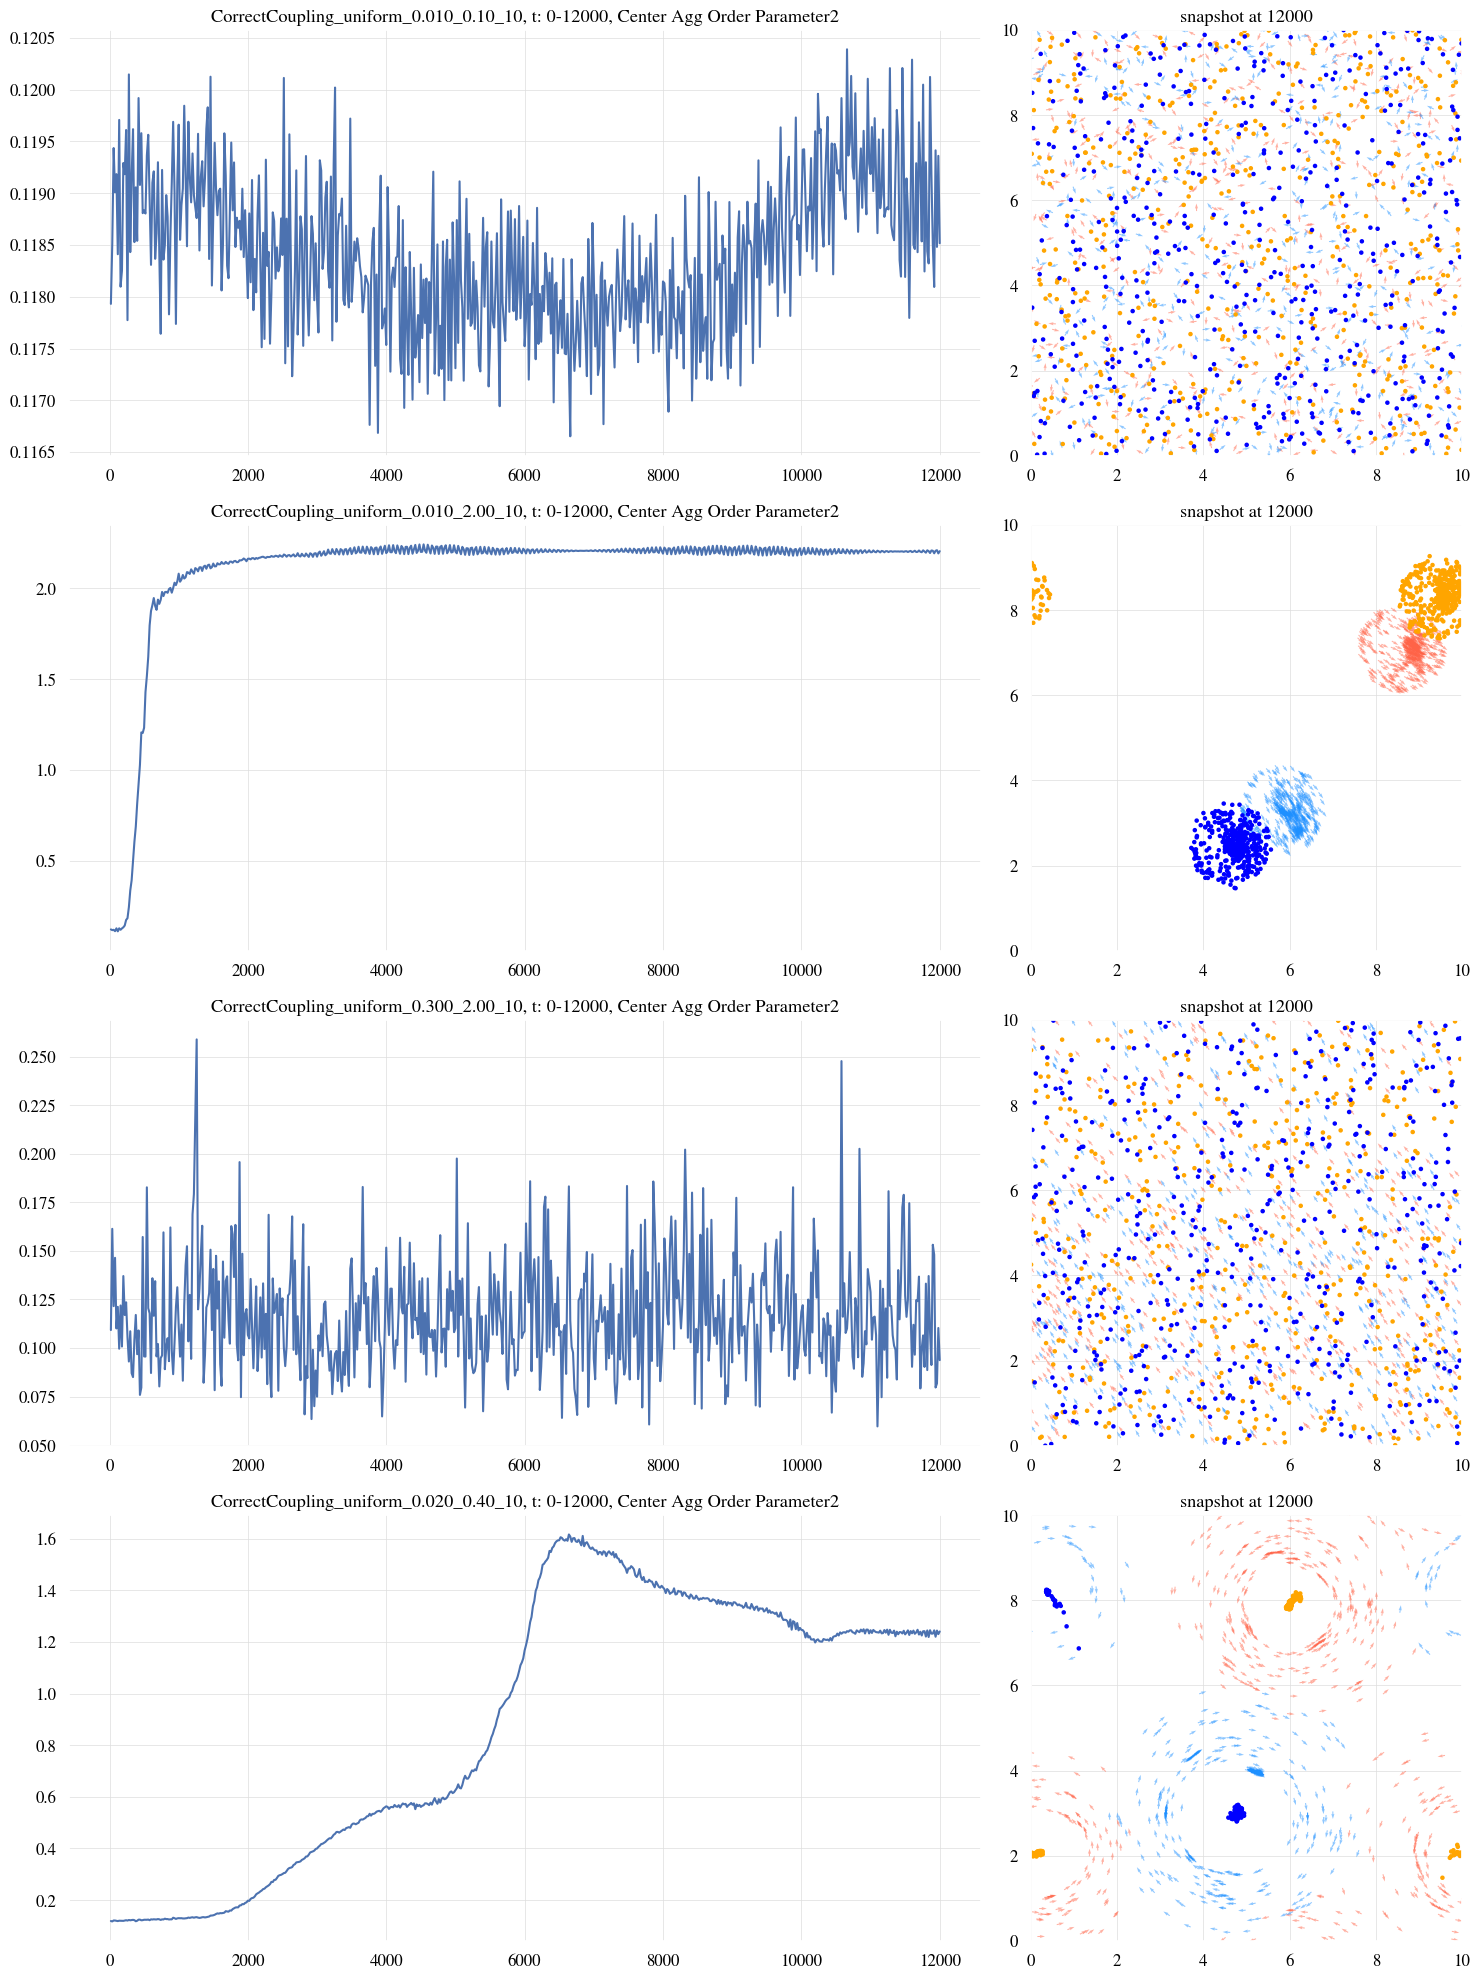
\includegraphics[width=0.9\textwidth]{./figs/centerAggOp2_ts.png}
	\vspace{-0.5cm}
	\caption{旋转中心空间聚集程度2}
	\label{fig:fig234t.5}
\end{figure}

\newpage
\noindent\textbf{旋转中心平均距离分布(时序序参量)}

将各粒子旋转中心与其余旋转中心的距离求平均,得到旋转中心平均距离分布,如下图所示:

$$
\bar{D}_i=\frac{1}{N}\sum_{j=1}^N{\bar{d}_{ij}}
$$

\begin{figure}[H]
	\centering
	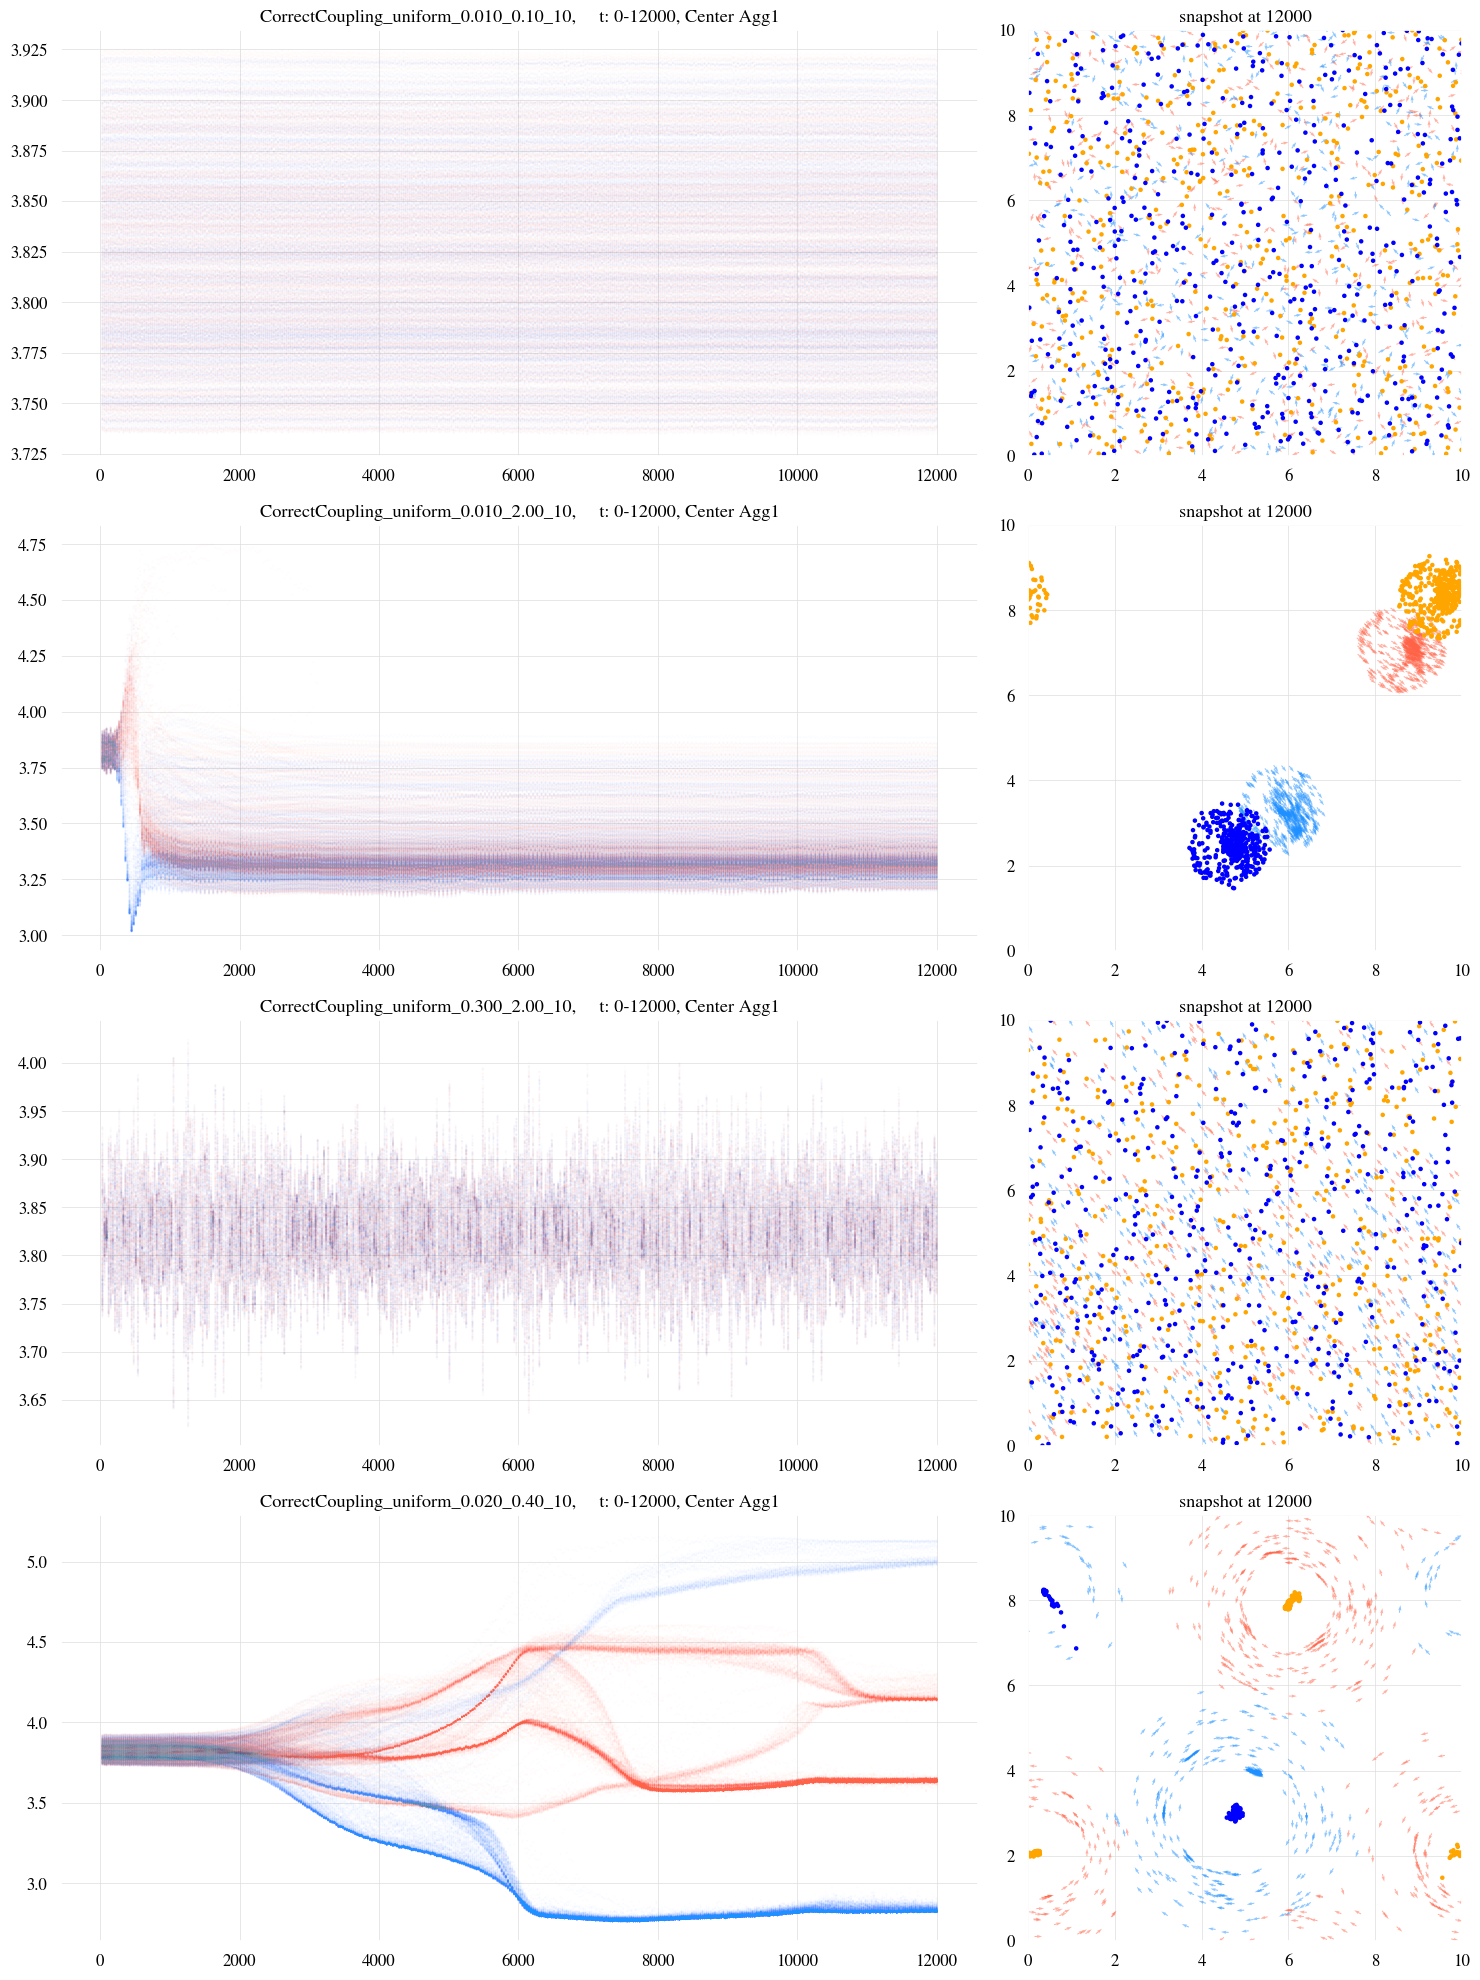
\includegraphics[width=0.9\textwidth]{./figs/centerAgg1_ts.png}
	\vspace{-0.5cm}
	\caption{旋转中心平均距离分布}
	\label{fig:fig234t.6}
\end{figure}

% \newpage

% \section{附录}\label{sec:appendix}

% \begin{figure}[H]
% 	\centering
% 	\includegraphics[width=\textwidth]{./figs/centorsBigGraph.png}
% 	\caption{旋转中心}
% 	\label{fig:fig2}
% \end{figure}

% \title{Swarm dynamics for oscillators with Phase Orientation Correlation}
% \maketitle

% \section{Introduction}

% \section{Results}
% \subsection{The Model}
% \subsection{Numerics}
% \subsection{Theoretical Analysis}


\end{document}